We'll begin our discussion of logic with the most primitive kind:
propositional\index{Logic!Propositional}.%
\footnote{%
    Also called \textit{sentential logic}\index{Logic!Sentential}.%
}
This deals with the structure of sentences, how the English language is used to
formulate arguments and deduce new facts. It is for this reason one should start
with the foundations of logic for at the heart of mathematics is the concept of
\textit{definition-theorem-proof}. The word definition, it is hoped, is
understood as a primitive of the English language (much like the word
\textit{the}) but theorem and proof require an explanation if we are to use them
consistently. We'll discuss propositions, predicates, implications, negations,
and overall what we are to consider valid reasoning. We return to logic later
in Books~\ref{book:Foundations} and \ref{book:Topology} when discussing
Boolean algebras\index{Boolean Algebra} and Stone spaces%
\index{Stone Space}\index{Topological Space!Stone Space}, culminating in Stone's
representation theorem.
\section{What is Logic?}
    It may seem strange to begin a study of mathematics with the development of
    logic as one might think such conversations should reside in philosophy.
    Indeed, most of classical logic was developed by philosophers rather than
    mathematicians. Many problems, which we will discuss in
    Chapt.~\ref{chapt:Zermelo_Fraenkel_Set_Theory}, arose in the early 1900s
    with the very core of mathematics. Arguments once considered sound were
    shattered and contradictions were discovered. On the other hand
    other methods of proof that are very intuitive were shown to be able to
    prove the existence of non-intuitive and almost impossible objects. This
    motivates us to develop the \textit{axioms}%
    \footnote{%
        The word axiom will be defined soon enough (Def.~\ref{def:Axiom}).
    }
    of logic and explore what valid arguments should look like.
    \begin{example}
        \label{ex:Logic_IVP}%
        A student of calculus has likely heard of the intermediate value
        theorem\index{Theorem!Intermediate Value}. Fear not those who haven't,
        we shall draw a picture. Given a \textit{continuous}%
        \footnote{%
            Intuitively a \textit{curve} one can draw from left to right without
            lifting up their pencil.%
        }
        function $f$ of real numbers, if $f(0)$ is negative and $f(1)$
        positive,%
        \footnote{%
            $f(0)$ means the evaluation of $f$ at zero. If $f$ has the formula
            $f(x)=x+1$, then $f(0)=1$.
        }
        then there is some point in the middle which evaluates to zero. The
        proof is quite simple: We first look at what happens to the point
        $\frac{1}{2}$. If $f$ is zero here we are done, otherwise if $f$ is
        positive then we may suspect there's a value in
        between 0 and $\frac{1}{2}$ which evaluates to zero and if $f$ is
        negative at this point, then there's probably a zero between
        $\frac{1}{2}$ and 1. In either case we divide the range of possibilities
        in half and see what happens at $\frac{1}{4}$ in the first case and
        $\frac{3}{4}$ in the latter. We continue \textit{inductively} (whatever
        this means) and obtain a \textit{sequence} of real numbers which we then
        show \textit{converges}. Invoking continuity, $f$ then evaluates to
        zero at this limit and we are done (see Fig.~\ref{fig:Sketch_of_IVP}).
    \end{example}
    \begin{figure}[H]
        \centering
        \captionsetup{type=figure}
        \if\compilefigures1
            \includegraphics{images/Intermediate_Value_Theorem_Sketch.pdf}
        \fi
        \caption{Sketch for the Intermediate Value Theorem}
        \label{fig:Sketch_of_IVP}
    \end{figure}
    We can see why this may work. After a few iterations we've narrowed down a
    zero point to a small range between $x_{3}$ and $x_{5}$ and this is a
    nice algorithm we can tell a computer to execute to arbitrary precision%
    \footnote{%
        This is known as the \textit{bisection} method%
        \index{Root Finding!Bisection}\index{Bisection Method} of root finding.%
    }
    but what went into the proof? If we are to phrase this with absolute rigor,
    what definitions, assumptions, and previous theorems are we relying on? For
    starters, the existence of \textit{real numbers}, a notion of
    \textit{continuity}, and the definition of a \textit{sequence}. Our
    exposition of logic is to make clear what is required for valid proofs.
    \begin{example}
        \label{ex:Logic_Gauss_Sum}%
        It has been alleged, though as always one should exhibit skepticism,
        that in 1784 at the age of seven the great mathematician Carl
        Friedrich Gauss\index{Gauss, Carl Friedrich} (1777-1855 C.E.)
        demonstrated that $1+2+\dots+99+100=5050$ \cite[p.~12-13]{von1856gauss}.
        It has also been claimed he had revelations about the normal
        distribution while counting the number of steps on his way to school,
        and that he corrected his fathers mathematical calculations at the age
        of three.%
        \footnote{%
            Many such claims were made by Gauss' biographer
            \textit{Wolfgang Sartorious von Waltershausen}, born 30 years after
            Gauss, publishing these stories in
            \textit{Gauss: zum Ged\"{a}chtnis}. Gauss apparently told some of
            these stories to von Waltershausen at old age in great excitement.
            It would be great to accept the tale as a feel-good story, but
            shortly after J\'{a}nos Bolyai
            (1802-1860 C.E.)\index{Bolyai, J\'{a}nos} published his account of
            absolute geometry in 1831 creating a common foundation for Euclidean
            and hyperbolic geometry, Gauss wrote that he was unable to give
            praise since he had developed these results 30 years prior but
            never published, offering no evidence of the claim. With such
            comments it is hard to tell what is factual about Gauss.
        }
        Alas, mathematicians are a few tales away from forming the religion of
        Gauss. Nevertheless, let's see what the argument is. We rearrange this
        sum as follows:
        \begin{table}[H]
            \centering
            \captionsetup{type=table}
            \begin{tabular}{ccccccccccc}
                &&$1$&$+$&$2$&$+$&$\cdots$&$+$&$99$&$+$&$100$\\
                \hline\\
                $=$&&$1$&$+$&$2$&$+$&$\cdots$&$+$&$49$&$+$&$50$\\
                &$+$&$100$&$+$&$99$&$+$&$\cdots$&$+$&$52$&$+$&$51$\\
                \hline\\
                $=$&&$101$&$+$&$101$&$+$&$\cdots$&$+$&$101$&$+$&$101$\\
                \hline\\
                $=$&&$50$&$\times$&$101$\\
                \hline\\
                $=$&&$5050$
            \end{tabular}
            \caption{Gauss' Sum of 1 to 100}
        \end{table}
        While this seems to be a concrete proof of the claim, is it valid? Can
        we generalize it? What assumptions about integers and arithmetic are we
        making?
    \end{example}
    \begin{example}
        \label{ex:Logic_Euler_Sum}%
        Gauss is often called the prince of Mathematics, and the king is the
        great Leonhard Euler\index{Euler, Leonhard} (1707-1783 C.E.). He too
        studied sums and considered the bizarre series $1+2+3+4+\cdots$ arriving
        at the answer $\minus\frac{1}{12}$.%
        \footnote{%
            While this sum was studied in the $18^{th}$ century, there seems to
            be ambiguity as to whether or not Euler earns the credit on this
            one. He writes this sum and others, such as $1+2+4+8+\cdots$ which
            he claims sums to $\minus{1}$ and $1+3+9+27+\cdots$ arriving at
            $\minus\frac{1}{2}$, in his text \textit{De Seriebus Divergentibus}
            (English: \textit{On Divergent Series}). He also computes Grandi's
            summation using the geometric series
            \cite[p.~206-208]{euler2012seriebus}. He does not sum $1+2+3+\cdots$
            to $\minus\frac{1}{12}$ like we do, only mentions it is probably
            negative.
        }
        Let's see how we can obtain this. First consider Grandi's
        series\index{Grandi's series}, named after Luigi Guido Grandi%
        \index{Grandi, Luigi Guido} (1671-1742 C.E.). We have:
        \begin{equation}
            G=1-1+1-1+1-1+\cdots
        \end{equation}
        Is there a meaningful number to assign to $G$? Suppose there is and
        write:
        \begin{table}[H]
            \centering
            \captionsetup{type=table}
            \begin{tabular}{rrrrrrrrrrrrr}
                $1-G$&$=$&$1$&$-$&$\Big[$$1$&$-$&$1$&$+$&$1$&$-$&$\cdots$
                    &$\Big]$\\[1ex]
                \hline\\
                    &$=$&$1$&$-$&$1$&$+$&$1$&$-$&$1$&$+$&$\cdots$\\[1ex]
                \hline\\
                &$=$&$G$
            \end{tabular}
            \caption{Grandi's Series $1-1+1-1+\cdots$}
        \end{table}
        \begin{minipage}[c]{0.58\textwidth}
            And hence we have $1-G=G$. Adding $G$ to both sides gives us $2G=1$,
            and after dividing by two we obtain $G=\frac{1}{2}$.
            Next, we consider the series:
            \begin{equation}
                T=1-2+3-4+5-6+\cdots
            \end{equation}
            This series was considered by Euler, writing it sums to
            $\frac{1}{4}$, admitting this is paradoxical since the first
            100 terms add to $\minus{50}$ and the first 101 terms sum to $+51$,
            neither of which is close to one-fourth. Nevertheless, we treat this
            series as we did Grandi's and see what can be done:
        \end{minipage}
        \hfill
        \begin{minipage}[c]{0.4\textwidth}
            \centering
            \begin{figure}[H]
                \centering
                \captionsetup{type=figure}
                \if\compilefigures1
                    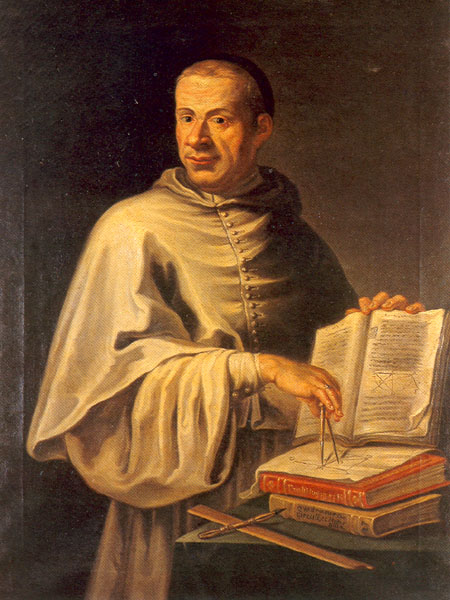
\includegraphics{photos/GuidoGrandi.jpg}
                \fi
                \caption{Luigi Guido Grandi}
                \label{photo:GuidoGrandi}
            \end{figure}
        \end{minipage}
        \begin{table}[H]
            \centering
            \captionsetup{type=table}
            \begin{tabular}{ccccccccccc}
                $2T$&$=$&$T$&$+$&$T$\\
                    \hline\\
                    &$=$&$1$&$-$&$2$&$+$&$3$&$-$&$4$&$+$&$\cdots$\\
                    &   &   &$+$&$1$&$-$&$2$&$+$&$3$&$-$&$\cdots$\\
                \hline\\
                    &$=$&$1$&$-$&$1$&$+$&$1$&$-$&$1$&$+$&$\cdots$\\
                \hline\\
                &$=$&$G$\\
                \hline\\
                &$=$&$\frac{1}{2}$
            \end{tabular}
            \caption{The Sum of $1-2+3-4+\cdots$}
        \end{table}
        That is, adding $T$ to itself gives us back Grandi's series which we
        know to be $G=\frac{1}{2}$. Hence, $2T=\frac{1}{2}$. Dividing by two
        gives us Euler's solution: $T=\frac{1}{4}$. We now return to Euler's sum
        which we'll denote $S$:
        \begin{equation}
            S=1+2+3+4+\cdots
        \end{equation}
        We subtract the series $T$ which we computed above, obtaining:
        \begin{table}[H]
            \centering
            \captionsetup{type=table}
            \begin{tabular}{ccccccccccccc}
                $S-T$&$=$&&       &$1$&$+$&$2$&$+$&$3$&$+$&$4$&$\cdots$\\
                     &&$-$&$\Big[$&$1$&$-$&$2$&$+$&$3$&$-$&$4$&$\cdots$&$\Big]$
                \\[1ex]
                \hline\\
                     &$=$&&&$0$&$+$&$4$&$+$&$0$&$+$&$8$&$\cdots$\\[1ex]
                \hline\\
                &$=$&&$4\Big[$&$1$&$+$&$2$&$+$&$3$&$+$&$4$&$\cdots$&$\Big]$
                    \\[1ex]
                \hline\\
                &$=$&&$4S$
            \end{tabular}
            \caption{The Sum of $1+2+3+4+\cdots$}
        \end{table}
        So $S-T=4S$. But $T=\frac{1}{4}$ and hence $3S=\minus\frac{1}{4}$.
        Thus $S=\minus\frac{1}{12}$.%
        \footnote{%
            The method of summation presented here is an augmentation of
            Srinivasa Ramanujan's (1887-1920 C.E.)\index{Ramanujan, Srinivasa}
            \cite[Chapt.~VIII p.~3]{RamanujanNotebooksI}.
        }
    \end{example}
    We now contemplate the previous examples and ask which are valid. It is
    tempting to say Ex.~\ref{ex:Logic_IVP} and Ex.~\ref{ex:Logic_Gauss_Sum} were
    presented with accurate proofs, whereas Ex.~\ref{ex:Logic_Euler_Sum} is
    garbage, but why? We ``proved'' Gauss' and Euler's sum in the same manner:
    Rearranged terms, used \textit{dot dot dot}%
    \footnote{
        As in $1+2+3+4+\cdots$ (\textit{dot dot dot}).
    }
    notation to indicate some pattern, added things together in a convincing
    way, and then simplified. One might suggest that Gauss' proof involved a
    finite scheme and that if asked one could laboriously write out the numbers
    indicated by the dots, whereas Euler's sum is infinite. But if we were to
    perform Gauss' problem with a number so large that it would take longer than
    the age of the universe to write down, even with the aid of computer, would
    we reject his method of proof then? There is some solace, and we can show
    that the Euler sum is invalid if we accept that $1\ne{0}$. Consider the sum
    $1+1+1+1+\cdots$ which we shall denote $B$ for bad. Using Grandi's series we
    subtract and obtain:
    \begin{table}[H]
        \centering
        \captionsetup{type=table}
        \begin{tabular}{ccccccccccccc}
            $B-G$&$=$&&       &$1$&$+$&$1$&$+$&$1$&$+$&$1$&$\cdots$\\
                 &&$-$&$\Big[$&$1$&$-$&$1$&$+$&$1$&$-$&$1$&$\cdots$&$\Big]$
            \\[1ex]
            \hline\\
                 &$=$&&&$0$&$+$&$2$&$+$&$0$&$+$&$2$&$\cdots$\\[1ex]
            \hline\\
            &$=$&&$2\Big[$&$1$&$+$&$1$&$+$&$1$&$+$&$1$&$\cdots$&$\Big]$
                \\[1ex]
            \hline\\
            &$=$&&$2B$
        \end{tabular}
        \caption{The Sum of $1+1+1+1+\cdots$}
    \end{table}
    And so we obtain $B-G=2B$, so $B=\minus{G}$. But we know Grandi's series is
    $G=\frac{1}{2}$, and hence $B=\minus\frac{1}{2}$. We can also do the
    following:
    \begin{equation}
        1+B=1+(1+1+1+1+\cdots)=1+1+1+1+\cdots=B
    \end{equation}
    And hence $1+B=B$, so $1=0$ which is a contradiction.
    \subsection{Truth}
        Since the aim of mathematics is to prove the validity of mathematical
        statements, we should start with a definition of truth\index{Truth}. We
        run into a wall instantly since this is essentially an impossible task.
        Any definition will be circular, and it is a theorem of
        Alfred Tarski\index{Tarski, Alfred} (1901-1983 C.E.) that if one has
        defined arithmetic, then one cannot use arithmetic to define
        truth.\index{Theorem!Tarski's Undefineability Theorem}%
        \index{Tarski's Undefineability Theorem}%
        \footnote{%
            This is known as Tarski's Undefineability Theorem.%
        }
        That is, if we take upon the assumption of the existence of the
        natural numbers 0, 1, 2, $\dots$ with the familiar notion of addition,%
        \footnote{%
            i.e. $1+1=2$ and other mathematical gems.
        }
        then \textit{arithmetic}%
        \footnote{%
            Pronounced \textit{eh-rith-meh-tik}.
        }
        truth cannot be defined using this arithmetic.%
        \footnote{%
            Pronounced \textit{ah-rith-muh-tik}. Isn't English fun?
        }
        \par\hfill\par
        Let us consult the dictionary. The Oxford English dictionary defines
        truth to mean \textit{in accordance with fact or reality}
        \cite{OEDTrueDef}, Merriam-Webster states that truth is
        \textit{the body of real things, events, and facts}
        \cite{MerriamWebsterTruthDef}, and Cambridge claims it is
        \textit{the quality of being true} \cite{CambridgeTruthDef}. As
        hypothesized these definitions are circular and rely on other predefined
        terms. We propose the following work around: Truth\index{Truth} is a
        primitive notion that needs no definition. We can then define
        false\index{False} to mean \textit{not} true.
        \par
        \begin{minipage}[c]{0.49\textwidth}
            \centering
            \begin{figure}[H]
                \centering
                \captionsetup{type=figure}
                \if\compilefigures1
                    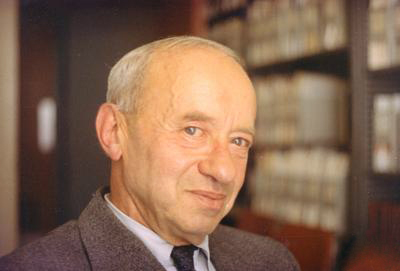
\includegraphics[scale=0.4]{photos/AlfredTarski1968.jpeg}
                \fi
                \caption{Alfred Tarski (1968, Colorized)}
                \label{photo:Alfred_Tarski}
            \end{figure}
        \end{minipage}
        \hfill
        \begin{minipage}[c]{0.49\textwidth}
            Tarski's result occured in the 1930's whilst trying to
            mathematically work out the
            \textit{liar's paradox}\index{Paradox!Liar's}\index{Liar's Paradox}
            \cite{TarskiUndefinability}. Consider the following sentence:
            \begin{equation}
                \text{This sentence is false.}
            \end{equation}
            Similar statements have been considered throughout the ages and
            it is mentioned twiced in the Christian Bible.
        \end{minipage}
        \par\vspace{2.5ex}
        One of the earliest renditions is known as Epimenides'
        paradox\index{Paradox!Epimenides'}.
        Epimenides of Cnossos (\textit{c.} 600 B.C.E.), who was from Crete,
        proclaims \textit{Cretans are always liars} \cite{KingJamesBible}. The
        question was considered again 200 years later when Eubulides of Miletus
        (\textit{c.} 400 B.C.E.) considered the sentence \textit{I am lying.}
        Further still in the Book of Psalms king David says
        \textit{I said in my haste, all men are liars} \cite{KingJamesBible}.
        Needless to say, the paradox is quite old and well studied. Now we ask,
        is the statement \textit{true} or \textit{false} (assuming such notions
        are defined)? Let's work through it and suppose truth. If this sentence
        is false is true, then the sentence is false even though we just claimed
        it to be true. Hence, it must be false. But if this sentence is false is
        false, then the sentence is true, but we just showed it cannot be true.
        So, which one is it? There are two interpretations: The statement is
        \textit{neither} true nor false, and the sentence is \textit{both} true
        and false. Suppose we accept that the statement is neither true nor
        false. This leads to another sentence where we cannot make such a
        conclusion:
        \begin{equation}
            \text{This sentence is not true.}
        \end{equation}
        If this is neither true nor false, then it is not true, and hence true,
        bringing us back to the paradox. Now we claim it is both true and false,
        leading us to:
        \begin{equation}
            \text{The sentence is false and not true.}
        \end{equation}
        The problem intensifies if we consider pairs of sentences:
        \twocolumneq[\par]{%
            \label{eqn:That_Sentence_Is_True}%
            \text{Statement \ref{eqn:That_Statement_Is_False} is true.}
        }
        {%
            \label{eqn:That_Statement_Is_False}%
            \text{Statement \ref{eqn:That_Sentence_Is_True} is false.}
        }
        and now we go round and round in an endless circle. As Alfred Tarski
        pointed out, the problem arises in languages in which statements are
        allowed to be self-referential. To see this is indeed a self
        referencing claim we write $P$ for the proposition and arrive at the
        equation:
        \begin{equation}
            P=P\text{ is false}
        \end{equation}
        if we substitute $P$, we obtain:
        \begin{equation}
            P=(P\text{ is false})\text{ is false}
             =\big((P\text{ is false})\text{ is false}\big)\text{ is false}
        \end{equation}
        While it may seem like this is an unnecessary discussion, the liar's
        paradox plays a role in mathematics. For one it motivates Tarski's
        theorem on the defineability of truth, and more famously it allowed Kurt
        G\"{o}del\index{G\"{o}del, Kurt} (1906-1978 C.E.) to prove his
        \textit{incompleteness theorems}, which really shook most of modern
        mathematics. Indeed, this theorem allegedly made Albert
        Einstein\index{Einstein, Albert} believe there could be no
        \textit{theory of everything}\index{Theory of Everything}.%
        \footnote{%
            A theory of physics that could solve all problems great and small.
            While no direct quotation from Einstein could be found, Stephen
            Hawking wrote that G\"{o}del's theorem convinced him no such theory
            can exist \cite{hawking2002godel}. Einstein was a close friend to
            G\"{o}del, which is probably connected to how this claim originated.
        }
        For the sake of moving on to mathematics we accept truth to be a
        primitive notion and acknowledge that the foundations of this concept
        are very shaky.
        \par\hfill\par
        Let us examine a few more paradoxes of the English language. The main
        troubles of set theory will have to wait until we've developed more
        vocabulary. The first to discuss is
        \textit{Berry's paradox}\index{Paradox!Berry's}\index{Berry's Paradox},
        named after G. G. Berry\index{Berry, G. G.} (1867-1928 C.E.), a junior
        librarian at one of Oxford's library who relayed the paradox to Bertrand
        Russell\index{Russell, Bertrand} \cite[p.~63]{CamCompBertRuss03}, who
        published it in 1906.%
        \footnote{%
            Berry's original paradox dealt with Cantor's theory of
            \textit{ordinal} numbers, not integers.
        }
        The paradox arises from the following sentence:
        \begin{center}
            \textit{The smallest positive integer not defineable in less than}
            \textit{60 letters}
        \end{center}
        This statement is itself only 57 characters long. The English language
        has 26 letters, a space bar, and 10 numerical symbols (in addition to
        grammatical symbols like commas), so let's suppose there are 50 distinct
        characters allowed in a sentence. There are then a total of
        $50^{60}\approx{8}\times{10}^{101}$ combinations. Just about all of
        these sentences are absolute gibberish, for example:
        \begin{center}
            \textit{qjasneofiq923m woasmd fd/'?maojs 3m ansdjf aia sdf iquer sj}
        \end{center}
        One of my more poetic works, called
        \textit{bashing my keyboard and counting to 60}. Some of these
        combinations of characters do indeed correspond to integers. For
        example, \textit{The smallest positive integer} is 1. In almost every
        system of arithmetic studied there exists a \textit{well-ordering}%
        \index{Well Ordering} property of the integers. If you are given a
        collection of positive integers and told it contains some number $n$,
        then there is a \textit{smallest} such. The proof is quite simple, ask
        yourself \textit{is 1 in the collection}? If yes, you are done since 1
        is the smallest positive integer, if not, proceed. Then ask
        \textit{is 2 in the collection}? Again, if yes then you are done since
        2 is the smallest positive integer greater than 1, but you've already
        checked that 1 is not in your collection. You continue until finally you
        hit an integer where the answer is \textit{yes}. You are guarenteed this
        process will stop since by hypothesis the collection has some integer
        $n$, and hence you need at most $n$ iterations of this procedure. This
        \textit{proof by algorithm} is not a proof unless we have some
        \textit{axiom} that such arguments are legal. Nevertheless it is
        intuitive and gives means of proving the claim in some theories (like
        Zermelo-Fraenkel Set Theory) and justifies accepting the principle as
        valid without requiring proof in others (like Peano Arithmetic).
        \par\hfill\par
        We use the well-ordering principle to formulate Berry's paradox. In
        mathematics we describe collections of objects with sentences. This need
        not be with English, but the problem will exist in any human language.
        For example,
        \textit{the collection of all integers which are divisible by two} is a
        description of the \textit{even} integers. So now we propose
        \textit{the set of all integers not defineable in less than 60 letters}.
        Since there are at most $\approx{10}^{102}$ such integers that are
        defineable in less than 60 characters, and since most presume there are
        infinitely many numbers, we conclude the collection of integers defined
        by this sentence is non-empty. Then by the well ordering principle there
        is a least such element. But then this least element satisfies the
        criterion \textit{The smallest positive integer not defineable in less}
        \textit{than 60 letters}, which is less than 60 letters. But we've
        described it in fewer than 60 characters, a contradiction.%
        \footnote{%
            Some number theorists use this paradox to prove all integers are
            interesting. If not, then there is a least such integer that is
            not interesting. But being the smallest boring integer is pretty
            interesting! Hence, all integers are interesting.%
        }
        \footnote{%
            There is a semantical equivalent more familiar to most (though
            almost all are unbothered by it). In the classic Disney movie
            \textit{Aladdin}, whilst singing the song
            \textit{A Whole New World}, princess Jasmine proclaims
            \textit{indescribable feeling}, and yet she just described it.
        }
        \par\hfill\par
        The resolution has already been alluded to. There is an ambiguity with
        the word \textit{defineable}. Does this sentence indeed define an
        integer? It seems the paradox merely gives a proof that it does not. One
        proposed alternative to this solution is to create a hierarchy. Hence
        \textit{The smallest positive integer that is not $defineable_{0}$}
        \textit{in less than 60 letters} is a number that is $defineable_{1}$ in
        less than 60 letters. Like the liar's paradox, Berry's has a role in
        mathematics. In 1989 the American mathematics George
        Boolos\index{Boolos, George}%
        \footnote{Note to be confused with George Boole.}
        used the paradox to prove G\"{o}del's incompleteness theorem in a
        different manner.
        \par\hfill\par
        Next is the \textit{Grelling-Nelson Paradox}%
        \index{Grelling-Nelson Paradox}\index{Paradox!Grelling-Nelson}. This is
        less mathematical than the previous one but has a familiar ring to it.
        It is named after the German logicians Kurt
        Grelling\index{Grelling, Kurt} (1886-1943 C.E.) and Leonard
        Nelson\index{Nelson, Leonard} (1882-1927 C.E.).%
        \footnote{%
            Nelson's great grandfather is the mathematician
            \textit{Johann Peter Gustav Lejeune Dirichlet}.%
            \index{Dirichlet, Peter Gustav Lejeune}
        }
        Label an adjective of the English language as \textit{autological} if
        whatever the adjective is describing also holds for the adjective
        itself. For example, \textit{polysyllabic} describes words with many
        syllables, of which polysyllabic is such a word. Even more creative,
        \textit{pentasyllabic} words have five syllables, which pentasyllabic
        happens to have. The word \textit{word} is autological, as is the word
        \textit{English} (so long as it's read in English). Label an adjective
        \textit{heterological} otherwise. The words \textit{monosyllabic} and
        \textit{long} are heterological. Now we consider the word heterological.
        Since this is an adjective it is valid to ask if it is autological or
        heterological. If we suppose it is heterological, then it describes
        itself and is thus autological, a contradiction. If it is autological
        then it describes itself, but heterological words do not describe
        themselves, a contradiction.
        \par\hfill\par
        The game  being played here is similar to the circularity of the
        liar's paradox. Since this problem is purely semantical, we move on to
        \textit{Curry's paradox}\index{Curry's Paradox}\index{Paradox!Curry's}.%
        \footnote{%
            Also known as L\"{o}b's paradox\index{Paradox!L\"{o}b's}%
            \index{L\"{o}b's Paradox}
        }
        Like the liar's paradox, this problem has mathematical use and is often
        seen as a simplification of the Kleene-Rosser paradox%
        \index{Kleene-Rosser Paradox}\index{Paradox!Kleene-Rosser} which was
        used to prove certain formal systems are inconsistent.%
        \footnote{%
            Much the way Russell's paradox proved na\"{i}ve set theory to
            be inconsistent.
        }
        The problem is named after the American mathematician
        Haskell Curry\index{Haskell Curry}%
        \footnote{%
            Programming enthusiasts should note the language
            \textit{Haskell} is named after Curry.
        }
        (1900-1982 C.E.).%
        \footnote{%
            Curry's paradox shows the inconsistentency of na\"{i}ve set theory,
            the original \textit{lambda calculus}, and Curry's
            \textit{combinatory logic}.
        }
        Let $P$ be any sentence, and let $Q$ be the sentence
        \textit{if this sentence is true, then P is true}. If $Q$ is true, then
        \textit{if this sentence is true, then P is true} is a true statment.
        Hence, $P$ is true. From this \textit{anything} can be proven. Like the
        liar's paradox the problem is in the allowance of self-referencing
        sentences. $Q$ can be written as the statement \textit{if Q, then P},
        which is certainly self-referential.
        \par\hfill\par
        We've quite a lot of cleaning up to do before we can delve into the core
        of mathematics. One might think this is a waste of time, but an
        inconsistent theory is truly horrible. The
        \textit{principle of explosion}\index{Principle of Explosion}%
        \footnote{We will prove the principle later in this chapter.}
        allows one to prove, given an inconsistent set of assumptions, that
        \textit{everything} is provably true and false. This is rather boring
        and something one would hope to avoid. While it will only play a small
        role throughout our investigations, we should discuss Bertrand
        Russell's\index{Russell, Bertrand} \textit{type theory}%
        \index{Type Theory}, invented in collaboration with
        Alfred North Whitehead\index{Whitehead, Alfred North}
        (1861-1947 C.E.).%
        \footnote{%
            Not to be confused with the great topologist J. H. C. Whitehead.
        }
        This was one of the first attempts at resolving these paradoxes. Here
        everything has a \textit{type}, which may be thought of as a
        non-negative integer. When discussing containment, for example
        \textit{the collection A is contained in the collection B}, we only
        give this meaning if $B$ is of type 1 greater than $A$. Operations can
        only be applied to objects of the correct type.
        \par\hfill\par
        Type theory has vast applications in computer science and programming.
        Programming languages like Python\index{Python} allow one to define
        functions that take in undefined inputs. The program will crash if an
        input is given that the function cannot safely handle. For example,
        consider the following code which is meant to take in a real number and
        add 1 to it:
        \par
        \begin{tcblisting}{
            before=\par\vspace{2ex},
            boxsep=0.5\topsep,
            after=\par\vspace{2ex},
            top=0ex,
            bottom=0ex,
            title=Python Code with Ambiguous Input,
            listing only,
            listing options={
                language=Python,
                basicstyle=\ttfamily,
                keywordstyle=\color{blue}\ttfamily,
                stringstyle=\color{red}\ttfamily,
                commentstyle=\color{green}\ttfamily,
                morecomment={[l][\color{magenta}]{\#}},
                numbers=left,
                framexleftmargin=-16ex,
                numbersep=-16ex,
                xleftmargin=-16ex
            }
        }
            def f(x):
                return x+1
        \end{tcblisting}
        If we enter $x=1$, then type $f(x)$, this will return 2 without error.
        However Python allows strings and if we enter $x=\textit{``Bob''}$ the
        program will crash. This implementation of type checking is called
        \textit{Duck typing}\index{Duck Typing}\index{Python}%
        \footnote{%
            If your input looks like a duck and sounds like a duck, it is
            probably a duck.
        }
        in which the type of the input is checked at run time and if the type
        looks correct, the program will attempt to execute it. Contrast this
        with languages which require types to be declared prior to compilation
        or executation. Writing this in C we have:%
        \index{C Programming Language}%
        \footnote{%
            For simplicity, \textit{double} in C simply means a real number.
        }
        \begin{tcblisting}{
            before=\par\vspace{2ex},
            boxsep=0.5\topsep,
            after=\par\vspace{2ex},
            top=0ex,
            bottom=0ex,
            title=C Code with Declared Input,
            listing only,
            listing options={
                language=C,
                basicstyle=\ttfamily,
                keywordstyle=\color{blue}\ttfamily,
                stringstyle=\color{red}\ttfamily,
                commentstyle=\color{green}\ttfamily,
                morecomment={[l][\color{magenta}]{\#}},
                numbers=left,
                framexleftmargin=-16ex,
                numbersep=-16ex,
                xleftmargin=-16ex
            }
        }
            double f(double x){
                return x+1;
            }
        \end{tcblisting}
        If we try to use this function on anything that is not a real number
        the program will refuse to compile.%
        \footnote{%
            Unless you're using a \textit{really} outdated compiler.
        }
        The entirety of type theory is laid out in the three volume
        treatise \textit{Principia Mathematica}. We will adopt Zermelo-Fraenkel
        set theory\index{Zermelo-Fraenkel Set Theory} in addition to the logical
        axioms of Hilbert\index{Hilbert, David} to formulate mathematics, both
        of which were introduced 20 years after Russell and Whitehead's efforts.
    \subsection{Sets}
        The main objects in mathematics are \textit{sets}. This development came
        about in the 1800's with figures like Georg Cantor\index{Cantor, Georg},
        Augustus De Morgan\index{De Morgan, Augustus}, and Bernard
        Bolzano\index{Bolzano, Bernard} making the first strides in the theory.
        The early history is intuitive, but vague. This led to Russell's
        paradox\index{Paradox!Russell's Paradox}\index{Russell's Paradox} which
        ultimately showed stricter axioms of set theory were needed. We
        currently only need a definition, and we will delve into the axioms in
        Chapt.~\ref{chapt:Zermelo_Fraenkel_Set_Theory}. Let's look to the
        primary source for a definition, posited by Georg Cantor
        (1845-1918 C.E.). He wrote \cite{Cantor1895}:
        \begin{center}
            \textit{A set is a gathering together into a whole of definite}
            \textit{distinct objects of our perception or of our thought, which}
            \textit{are called the elements of the set.}
            \par\hfill
            \textit{Beitr\"{a}ge zur Begr\"{u}ndung der Transfiniten}
            \textit{Mengenlehre}%
            \footnote{%
                English:
                \textit{Contributions in Support of Transfinite Set Theory}.%
            }
            \par\hfill
            \textit{Georg Cantor, 1985 C.E.}
        \end{center}
        Felix Hausdorff\index{Hausdorff, Felix} (1868-1942 C.E.) posits
        \cite[p.~11]{HausdorffSetTheory}:
        \begin{center}
            \textit{A set is formed by the grouping together of single objects}
            \textit{into a whole. A set is a plurality thought of as a unit.}
            \par\hfill
            \textit{Mengenlehre}%
            \footnote{%
                English:
                \textit{Set Theory}.%
            }
            \par\hfill
            \textit{Felix Hausdorff, 1927 C.E.}
        \end{center}
        Both are beautifully phrased, but circular since the terms
        \textit{gathering}, \textit{objects}, and \textit{grouping} are not
        defined. This form of circularity was addressed by Alfred Tarski in his
        1946 book \textit{Introduction to Logic and the Methodology of the}
        \textit{Deductive Science}. He expresses the need for primitive
        undefined notions that we take for granted and use freely. We collect
        the smallest number of primitives possible, motivated by intuition, and
        then define other terms in our theory by means of sentences involving
        these primitives and previously defined terms.
        \par\hfill\par
        I do not wish to imply the circularity of the foundations of
        mathematics was created with the advent of set theory. In what is
        perhaps the most important textbook ever written,
        \textit{The Elements}\index{Elements, The (Euclid)} by Euclid of
        Alexandria (\textit{c.} 300 B.C.E), we find the first known work
        that employs the \textit{axiomatic method}\index{Axiomatic Method}. It
        starts with definitions, \textit{postulates}, and
        \textit{common notions}, and proceeds to prove a plethora of important
        theorems in a logical manner deriving results from these primitives and
        previously proved theorems. In modern language postulates and common
        notions are known as \textit{axioms}, which are statements that we
        accept as true without evidence or proof. It is not without flaw since
        his primitive definitions are circular. For example, the
        first definition is of a point:
        \begin{center}
            \textit{A point is that which has no part.}
            \par
            \hfill\textit{The Elements}\par
            \hfill\textit{Euclid of Alexandria, c. 300 B.C.E.}
        \end{center}
        The word part is never defined. Similarly, a line is defined as
        \textit{breadthless length}. This is not to detract from his efforts but
        to show the problem of \textit{infinite regress}\index{Infinite Regress}
        is unavoidable unless we assert that certain terms need no definition.
        For us, the word set will have no real definition. Nevertheless, we
        write the following:
        \begin{fdefinition}{Set}{Set}
            A \gls{set} is a collection of objects called the elements of the
            set.\index{Set}\index{Set!Definition}
        \end{fdefinition}
        The circularity we pointed out in Cantor's definition arises here since
        neither \textit{collection} nor \textit{object} have been defined. To
        begin doing mathematics we need a \textit{thing}. Sets act as our thing.
        We know they exist%
        \footnote{%
            In the sense of Plato's realism.%
            \index{Plato}\index{Platonic Realism}
            Whether sets exist in any real sense is another question.
        }
        but cannot define them very well. Instead we describe how they behave
        and how to obtain new sets from pre-existing ones via \textit{axioms}.
        Before doing so we should first get familiar with the notation. We
        cannot build set theory just yet since we've yet to develop logic. In
        the most elementary systems such as Peano arithmetic there is a notion
        of set, and hence we need to define this first. Pedagogically it is poor
        to proceed without examples, so we provide some now.
        \begin{fnotation}{Element Notation}{Element_Notation}
            If $A$ is a \gls{set} and if $x$ is an element\index{Set!Element of}
            of $A$, then we denote this by writing
            \glslink{containmentsymb}{$x\in{A}$}. If $x$ is not an element
            of $A$, we write $x\notin{A}$.\index{Containment $\in$}%
            \index{Element}\index{Element!Notation}
        \end{fnotation}
        \begin{example}
            The first three letters of the Latin alphabet can be expressed in
            set notation as follows. If we let the symbol $A$ denote this set, we
            may write:
            \begin{equation}
                A=\{\,a,\,b,\,c\,\}
            \end{equation}
            This is the standard for smaller sets; separate the elements by
            commas and enclose with braces. Letting $B$ denote the first three
            positive integers, we get:
            \begin{equation}
                B=\{\,1,\,2,\,3\,\}
            \end{equation}
            Using element notation (Not.~\ref{not:Element_Notation}) we have
            $1\in{B}$, but $4\notin{B}$. That is, $B$ contains the number 1 but
            does not contain the number 4. Similarly, $a\in{A}$ and
            $d\notin{A}$. The symbol $\in$ reads \textit{is in}, or
            \textit{is an element of}, or \textit{is contained inside of}. Thus
            $a\in{A}$ reads $a$ is an element of $A$, or simply $a$ is in $A$.
            The notation $\notin$ is the negation of this: \textit{not in} or
            \textit{not an element of}. Hence $4\notin{B}$ reads
            4\textit{ is not an element of B}, or 4\textit{ is not in B}.
        \end{example}
        \begin{example}
            For the working mathematician sets are allowed to contain almost
            anything they like. For example, we could consider the set of all
            cities of Earth and label this $C$. Then Boston is an element of
            $C$, but Massachusetts is not since Boston is a city, but
            Massachusetts is not (it's a state). Similarly, London would be an
            element of $C$, but England would not be.
        \end{example}
        As we've seen, it is common to denote small sets be enumerating all of
        the elements, separating with commas, and then enclosing in braces.
        Rigorously we need to justify such notation with axioms, such as the
        \textit{axiom of pairing}, which asserts the existence of sets like this
        but for now it's safe to just present this as what finite sets are. It
        is important to note the distinction between $A$ and $\{A\}$ since these
        are not the same thing%
        \footnote{%
            Provably so using the axiom of a regularity, so this claim is by no
            means obvious.
        }
        much the way there is a difference between a human and the house that
        human lives in.
        \begin{example}
            \label{ex:Everything_is_a_Set}%
            In the set theory that we will be working with, Zermelo-Fraenkel set
            theory\index{Zermelo-Fraenkel Set Theory}, abbreviated
            \gls{ZFC}, \textit{everything} is a set. This will be explained
            later, but we quite literally mean everything. The integers will be
            defined via John von Neumann's\index{von Neumann, John}
            construction. We start with the empty set\index{Empty Set}
            $\emptyset$ which is the set that contains nothing, often denoted
            $\emptyset=\{\,\}$, and this will be our zero. We proceed and define
            $1=\{\emptyset\}$, $2=\{\emptyset,\{\emptyset\}\}$,
            $3=\{\emptyset,\{\emptyset\},\{\emptyset,\{\emptyset\}\}\}$, and so
            on. This can be written more attractively as $0=\{\}$, $1=\{0\}$,
            $2=\{0,1\}$, and $3=\{0,1,2\}$, and hence $n$ is just a set
            containing $n$ things using our usual intuitive notion of counting.
            Moreover \textit{functions} are defined as sets, as are
            \textit{ordered pairs} $(a,b)$, and even \textit{orderings}. The
            examples presented here, such as sets of letters, sets of cities,
            etc., are for the sake of intuition and familiarization. No claim is
            made that these are actual sets in a mathematically rigorous sense.
            In ZFC everything is a set, the elements of a set are sets
            themselves, as are the elements of those elements, and so on,
            creating massive towers of sets. The axioms of ZFC are laid out to
            ensure these towers don't collapse on themselves with
            contradictions.
        \end{example}
        While in \gls{ZFC} we do adopt the idea that everything is a set, there
        seems to be universal agreement about notation for sets. Capital Latin
        letters like $A,B,C,X,Y,Z$ denote sets that we actually want to think of
        as collections of things, whereas lowercase Latin letters like
        $a,b,c,x,y,z$ denote elements of these sets which we think of as
        ordinary mathematical objects like numbers, or functions, or whatever.
        Because of this it often causes one discomfort where in the proof of
        something we need to write $x\in{y}$. This is especially true in the
        development of arithmetic. The benefit of the construction described
        above is we now have a simple means of \textit{ordering} the integers
        and we can write $m<n$ (read as \textit{m is less than n}) if it is true
        that $m\in{n}$. But this leads to the bizarre notation $1\in{2}$ or
        $0\in{3}$, which may cause some anxiety.
        \begin{example}
            The collection of all non-negative integers $0,1,2,\dots$ constitute
            a set which is often denoted $\mathbb{N}$. If we include the
            negatives we also get a set, labelled $\mathbb{Z}$. The rational
            numbers form a set, as do the real numbers, and these are written
            $\mathbb{Q}$ and $\mathbb{R}$, respectively. Lastly, the complex
            numbers also create a set $\mathbb{C}$. It is not obvious how to
            make these familiar things into sets without circularity, something
            we wish to avoid in foundations. Such constructions are another aim
            of Book~\ref{book:Foundations}.
        \end{example}
        Elaborating on the discussion in Ex.~\ref{ex:Everything_is_a_Set}, there
        are other theories for the foundations of mathematics that allow for
        primitive notions such as classes and universes. Some of these theories
        are extremely weak (cannot prove much) but very safe (there is likely no
        contradiction), whereas some are very user friendly but almost certainly
        fallacious. Peano's axioms are an example of a weak system of which the
        axioms are so basic and obvious that no one is likely to ever find a
        contradiction, but they cannot assert the existence of negative
        integers, let alone the reals. On the other hand, any theory that
        allows one to say the \textit{collection} of all sets whether the
        collection is a class, or a universe, or whatever, is one that should be
        treated with skepticism. The theory of Zermelo and Fraenkel is a healthy
        middle ground. Strong enough to do most mathematics, and no
        contradiction found yet, though much of the $20^{th}$ century was spent
        searching to no avail.
        \subsubsection{A Brief History}
            Considering collections of things and naming them accordingly dates
            back to antiquity. Aggragates of points are defined in Euclid's
            elements and large assemblages have been used in mathematics since.
            The term \textit{set} seems to appear first in the works of
            Bernard Placidus Johann Nepomuk Bolzano (1781-1848 C.E.), a Bohemian
            who coined the German term \textit{Menge}, which translates to set
            in English\index{Bolzano, Bernard}. The phrase appears in his
            \textit{Paradoxien des Unendiichen}%
            \footnote{%
                English: \textit{The Paradoxes of the Infinite}.
            }
            which was posthumously published in 1851. At the time Bolzano was
            known mostly for his philosophical works, including his 1837
            \textit{Wissenschaftslehre}%
            \footnote{%
                English: \textit{Theory of Science}.
            }
            which attempts to provide a logical foundation to the natural
            sciences. It is a shame, then, that he did not enjoy the fame as a
            mathematician accredited to him today since his groundbreaking works
            in real analysis were not published until the 1880's when the
            Austrian mathematician Otto Stolz\index{Stolz, Otto}
            (1842-1905 C.E.) happened across Bolzano's journals.
            \par\hfill\par
            Alluded to in Bolzano's text is \textit{Galileo's Paradox}%
            \index{Galileo's Paradox}\index{Paradox!Galileo's} put forward by
            the famed Italian astronomer Galileo Galilei\index{Galilei, Galileo}
            (1564-1642 C.E.)%
            \footnote{%
                In one of the \textit{faux} coincidences of history, Galileo
                Galilei died the same year Sir Isaac Newton was born
                (1642-1727 C.E.). One must use the \textit{Julian} calendar for
                Newton and the \textit{Gregorian} for Galileo. Using the
                Julian for Galileo puts his death in 1641, and Newton was born
                in 1643 using the Gregorian, somewhat ruining this
                \textit{coincidence}. However, $17^{th}$ century England used
                the Julian, and $17^{th}$ century Italy used the Gregorian, so
                the claim is not entirely bogus.
            }
            in his work \textit{Discorsi e Dimostrazioni}
            \textit{Matematiche Intorno a Due Nuove Scienze},%
            \footnote{%
                English: \textit{Discourses and Mathematical Demonstrations}
                \textit{Relating to Two New Sciences}.
            }
            usually referred to as \textit{two new sciences}. The paradox is
            formally resolved in set theory, most notably in the works of Georg
            Cantor in the late 1800's. Quite impressive, then, that Galileo
            pondered such problems two centuries ahead of his time.
            \begin{figure}[H]
                \centering
                \captionsetup{type=figure}
                \if\compilefigures1
                    \includegraphics{images/Galileo_Paradox_001.pdf}
                \fi
                \caption{Lines for Galileo's Paradox}
                \label{fig:Galileo_Paradox_001}
            \end{figure}
            Consider the two lines drawn in Fig.~\ref{fig:Galileo_Paradox_001}.
            One is longer than the other but both contain infinitely many
            points. Since one is greater we are forced to conclude, as Galileo
            wrote, that we have something greater than infinity since the
            infinity of points in the longer is greater than the infinity of
            points in the shorter \cite{GalileoTwoNewSciences}. The conclusion
            is somewhat correct, there are different infinities in set theory.
            The infinity of the real numbers is strictly greater than the
            infinity of the natural numbers, for example. This will be made very
            clear when we discuss bijective functions and cardinalities, but for
            now it may seem as mathematical gibberish.%
            \footnote{%
                These conclusions are due to Cantor. Some, like Hilbert,
                defended his work while many, like Kronecker and Wittgenstein,
                lambasted his writings and his character. Some solace: Most of
                Cantor's works were accepted as true by the mid $20^{th}$
                century and his results have become standard in $21^{st}$
                century analysis, topology, and measure theory courses.
            }
            Galileo is wrong in claiming one line has more points than the other
            since both have the same infinity of points. That is, we can match
            up every point of the long line to a unique point in the short line,
            showing the longer one can't be greater in quantity.
            \begin{figure}[H]
                \centering
                \captionsetup{type=figure}
                \if\compilefigures1
                    \includegraphics{images/Galileo_Paradox_002.pdf}
                \fi
                \caption{Solution to Galileo's Paradox}
                \label{fig:Galileo_Paradox_002}
            \end{figure}
            To construct this one-to-one correspondence requires a bit of
            perspective. Suppose we place an observer at the point $O$ shown in
            Fig.~\ref{fig:Galileo_Paradox_002}. The observer would not see the
            longer line, but if he or she were able to then both would appear to
            be the same length. To get our one-to-one correspondence we draw a
            straight line from this observer to the first line and then continue
            outwards to the longer one. This takes a point in the short line
            uniquely to a point in the long one, and every point in the long
            line is hit by some point in the short one. So we've matched every
            point in the short line to every point in the long line and hence
            the claim cannot be made that one has \textit{more} elements than
            the other. What sets them apart (their \textit{length}) is not a
            set-theoretic concept, but rather a \textit{measure} theoretic one.%
            \footnote{%
                In a late night musing I stumbled across this same problem. I
                learned of the solution from my mathematical mentor James
                \textit{Kiwi} Graham-Eagle who presented me with
                Fig.~\ref{fig:Galileo_Paradox_002}.
            }
            \par\hfill\par
            Galileo's second paradox is presented in a similar manner. He writes
            that there are infinitely many integers, and infinitely many square
            integers. Every square integer is also an integer, for example 1, 4,
            9, 16, 25, and so on. The converse is false, not every integer is a
            square integer since 2, 3, 5, 6, 7, 8, 10, and so on are not
            squares. From this argument Galileo concluded there are
            \textit{more} integers than square integers. The following
            observation then troubled him. For every integer%
            \footnote{%
                Here we loosely use integer to mean non-negative natural number:
                0, 1, 2, 3, etc.
            }
            there is a unique square number, namely given $n$ there is $n^{2}$.
            Given this there cannot be more integers than squares, a
            contradiction.
            \par\hfill\par
            The amazing part about this paradox is that it already contains its
            own solution. The \textit{function} which sends $n$ to $n^{2}$ is a
            \textit{bijection} between the integers and the squares. In set
            theory if a bijection exists, then the two sets have the same
            size. The problem can be reduced significantly if we note that not
            every integer is even, but every even integer is an integer. One
            might wrongly conclude then that there are more integers then even
            integers. But for every integer there is precisely one even integer,
            namely given $n$ we have $2n$. Even easier, all positive integers
            are integers, but not all integers are positive since zero is not
            positive. We might then conclude that the set of positive integers
            has infinity points, whereas the set of all integers has infinity
            + 1 points. But for every integer there is precisely one positive
            integer, namely given $n$ we have $n+1$.
            \par\hfill\par
            All three examples have the same problem. We take an infinite set,
            remove points%
            \footnote{%
                Perhaps infinitely many, as Galileo did.
            }
            but arrive at a set that is the same \textit{size} as what we
            started with. As stated, this problem is handled in set theory. By
            definition two sets are of the same size if a one-to-one
            correspondence (like $n\mapsto{n}^{2}$ or $n\mapsto{2n}$ or
            $n\mapsto{n}+1$)%
            \footnote{%
                The symbol $\mapsto$ reads aloud as \textit{maps to}.
            }
            exists between them. What's even more troubling%
            \footnote{%
                Unbeknownst to Galileo but knowst to Cantor.
            }
            is that the set of all \textit{rational} numbers is the same size as
            all of these. We'll explore this rigorously in
            Chapt.~\ref{chapt:Cardinality}.
    \subsection{Predicates and Propositions}
        Propositions and predicates will be two more of our primitive notions
        which we will vaguely define, but mostly rely on intuition.
        \begin{fdefinition}{Predicate}{Predicate}
            A \gls{predicate} $P$ on a \gls{set} $A$ is a sentence such that for
            all $x\in{A}$ one may state that $P(x)$ is either true or false.%
            \index{Predicate}\index{Predicate!Definition}
        \end{fdefinition}
        We have technically left the realm of propositional logical and entered
        \textit{predicate logic}\index{Predicate Logic}\index{Logic!Predicate}.
        This is because we needed to \textit{quantify} over all of the elements
        of the set $A$. That is, we've used the phrase \textit{for all}, a type
        of quantifier that is dealt with in predicate logic, not propositional.
        In strict propositional logic we would define \textit{propositional}
        \textit{variables}\index{Propositional Variable}, which is a primitive
        taken to be a variable which can either be true or false. These are also
        called \textit{atomic formulae}\index{Atomic Formula}, and from some set
        $A$ of atomic formulae one obtains a language by combining these
        primitive variables with logical \textit{connectives} such as $\neg$,
        $\land$, $\lor$, $\Rightarrow$, and $\Leftrightarrow$, each of which
        we'll discuss in the next section. So if $A$ is our set of propositional
        variables, and if $p,q\in{A}$, then $p\land{q}$ is something valled a
        \textit{well-formed formula}. A language is then obtained by considering
        the set of all well-formed formulae that are obtained using the
        following three rules:
        \begin{itemize}
            \item[1.)] If $p\in{A}$ is an atomic formula, then it is a
                       well-formed formula.
            \item[2.)] If $p\in{A}$ is an atomic formula, then $\neg{p}$ is a
                       well-formed formula. 
            \item[3.)] If $p,q$ are well-formed formulae, and if $b$ is a
                       logical connective, then $pbq$ is a well-formed formula.  
        \end{itemize}
        We will not completely abandon propositional logic but since we will,
        as all mathematicians must, accept predicate logic into our vocabulary
        there is no harm in introducing Def.~\ref{def:Predicate} now. It is,
        after all, a primitive definition. For pure propositional logic one may
        consider as the set of propositional variables the sentences
        $P(x)$ for all $x\in{A}$. These are then just sentences which one may
        ask \textit{is it true or false}, which is precisely what a
        propositional variable is.
        \par\hfill\par
        Predicates are the main tool used in set theory for defining and
        building new sets via the \textit{axiom schema of specification}%
        \index{Axiom!Schema of Specification}. Many describe predicates as
        \textit{functions} from a set $A$ to the Boolean-valued set
        $\{\text{True},\,\text{False}\}$, which is fine provided the notion
        function has been defined. To do so now would requires us to make
        \textit{function} another primitive, and thus one has the following
        problem: Do we accept \textit{predicate} as a primitive, or
        \textit{function}? Since predicates are essentially just sentences,
        we'll adopt these as primitives and later \textit{define} functions
        using elementary notions from the axioms of set theory.
        \par\hfill\par
        To see if our definition matches other standards, let's consult a
        dictionary and a textbook. Merriam-Webster writes that a predicate is
        \textit{something that is affirmed or denied of the subject in a}
        \textit{proposition in logic} \cite{MerriamWebsterPredicateDef}. This is
        a linguistic definition for the use of word predicate in English,
        whereas mathematicians often use overly convoluted formulas to define
        things. Looking to Cunningham's \textit{A Logical Introduction to Proof}
        we have that \textit{A predicate is just a statement proclaiming that}
        \textit{certain variables satisfy a property}
        \cite{Cunningham2010}. He then uses the example \textit{x is tall} where
        $x$ is taken to be a variable. Thus our adopted definition is not at all
        different from the linguistical or mathematical ones, and it truly is a
        primitive notion.
        \begin{example}
            Let $A$ be the set $A=\{1,2,3\}$ and let $P$ be the predicate
            \textit{x is greater than 2}. To be precise, $P$ is a predicate on
            the set of all positive integers 1, 2, 3, 4, etc. The set of values
            in $A$ which satisfy $P$ is $B=\{3\}$. If we let $Q$ represent
            \textit{x is negative}, then there are no elements in $A$ that
            satify $Q$ and hence the resulting set is the empty set $\emptyset$.
        \end{example}
        \begin{example}
            Let $X$ be any set and let $P$ be the sentence $x$ is not equal to
            $x$. There are no elements which satisfy this criterion and hence
            the sentence is always false for any input $x$. In other words, the
            set of elements which satisfies $P$ is the empty set $\emptyset$.
            A sentence that is always false is called a
            \textit{contradiction}.\index{Contradiction}
        \end{example}
        This is the primary means of forming sets in mathematics. We take a set
        we have proven exists and then apply some sentence to it and collect all
        elements of the set satisfying our statement. To do this requires
        justification, and this is the \textit{axiom schema of specification}.
        For example, if we have $A=\{1,2,3\}$ and $P$ is the predicate on $A$
        claiming \textit{x is greater than 2}, then we form a new set $B$ by
        collecting the elements of $A$ which satisfy $P$. We denote this using
        the so-called \textit{set-builder notation}\index{Set-Builder Notation}%
        \index{Set!Set-Builder Notation}:
        \begin{equation}
            B=\{\,x\in{A}\;|\;P(x)\,\}
        \end{equation}
        In more relaxed settings one uses the \textit{axiom of unrestricted}
        \textit{comprehension}\index{Axiom!of Unrestricted Comprehension} which
        allows one to form a set by any sentence. That is, we need not first
        consider some set $A$ and then apply our sentence $P$ to the elements of
        $A$ and extract the elements $x\in{A}$ which satisfy $P$, instead we
        ask for the \textit{set of all things satisfying P}. That is, we write:
        \begin{equation}
            B=\{\,x\;|\;P(x)\,\}
        \end{equation}
        Unfortunately this leads to contradiction and must be avoided.
        Nevertheless it is common in textbooks on measure theory or analysis,
        where convoluted sets need to be constructed, to appeal to unrestricted
        comprehension regardless of the consequences. It is fortunate enough
        that almost all of these constructions can be reformulated in a manner
        consistent with \gls{ZFC}.
        \par\hfill\par
        Moving on to propositions, we first express the Aristotelian
        definition put forward by Aristotle\index{Aristotle} (384-322 B.C.E.).
        \begin{equation}
            \text{A proposition is a sentence which affirms or denies a }
            \text{predicate.}
        \end{equation}
        Examples of propositions are found in the so-called
        \textit{Socrates syllogism}\index{Socrates!Syllogism of}.
        \begin{example}
            We wish to conclude the ancient greek philosopher
            Socrates\index{Socrates} was mortal. We start with the following
            proposition: \textit{All men are mortal}. We assert this sentence is
            true and may be used later in the proofs of other claims. Second,
            we state \textit{Socrates is a man}. This is another proposition
            that we accept as true. To conclude Socrates is mortal we need some
            \textit{rule of inference} that allows us to tie these two
            propositions together. One such rule, known as
            \textit{modus ponens}\index{Modus Ponens}%
            \index{Axiom!of Modus Ponens}, does what we need. It states
            that if $P$ and $Q$ are propositions, if $P$ implies $Q$, and if $P$
            is true, then $Q$ is true. Using this, since all men are mortal, and
            since Socrates is a man, we conclude that Socrates is mortal.
        \end{example}
        An easier proof that Socrates is mortal goes as follows: He's dead.
        Nevertheless, we are starting to see what is needed to construct valid
        proofs. We formalize the Aristotelian view slightly, adopting the
        following definition:%
        \footnote{%
            Though recognizing that this is again another primitive.
        }
        \begin{fdefinition}{Proposition}{Proposition}
            A \gls{proposition} is a \gls{predicate} on a \gls{set} $A$
            evaluated at a particular element $x\in{A}$, which is then affirmed
            or denied to be true.%
            \index{Proposition}\index{Proposition!Definition}
        \end{fdefinition}
        What if we have a proposition that takes in several variables? Moreover,
        how do we respect the order of the input when dealing with more than one
        variable? From how we've defined predicates and propositions the input
        is a single element of the set $A$. To speak of \textit{multivariable}
        predicates and propositions requires order, which sets do not have.
        Indeed, the only distinguishing feature of a set is the elements it
        contains and hence $\{1,2,3\}$ and $\{3,2,1\}$ are identical. Ordering
        sets is a big part of elementary set theory and is dealt with by
        constructing the \textit{Cartesian Product}\index{Cartesian Product} of
        two sets. Since we do not have such notions at the moment our predicates
        must act on single variables.
        \begin{example}
            Let's use the previous example of Socrates to motivate what we mean.
            Let $P$ be the predicate \textit{x is a man}.%
            \footnote{%
                To be precise, it is a predicate on the set of all humans who
                have ever lived.
            }
            If we input Socrates we obtain $P(\text{Socrates})=\text{True}$. If
            we input Hatshepsut, we get $P(\text{Hatshepsut})=\text{False}$.
            This is how we distinguish a predicate from a proposition. $P$ is
            a predicate, whereas $P(\text{Hatshepsut})=\text{False}$ is
            proposition.
        \end{example}
        \begin{example}
            Suppose we have invented the notion of ordered pairs somehow, and
            we denote this by $(x,y)$ using parentheses. So $(x,y)$ and $(y,x)$
            are distinct things whenever $x$ and $y$ are different. With this,
            let us consider the predicate \textit{x is a man, y is a woman} and
            let us label this $P\big((x,y)\big)$.%
            \footnote{%
                As pointed out in Halmos' text, while $P\big((x,y)\big)$ is the
                \textit{correct} notation, $P$ accepts ordered pairs as input,
                everyone just writes $P(x,y)$ \cite[p.~32]{Halmos1974}.
            }
            \footnote{%
                To be precise, $P$ is a predicate on the set of all
                \textit{ordered pairs} of humans.
            }
            The \textit{order} of the inputs now
            matters. For example,
            $P(\text{Socrates},\text{Hatshepsut})=\text{True}$, but
            $P(\text{Hatshepsut},\text{Socrates})=\text{False}$.
        \end{example}
    \subsection{Rules of Inference}
        Given a collection of propositions we often wish to derive new ones.
        Indeed, that is the entirety of mathematics: Proving new theorems. We
        must precisely state which rules we accept as valid and then attempt to
        stay consistent with them. The first we have already discussed,
        \textit{modus ponens}. This rule applies to \textit{implications}, one
        of the two primitives we adopt in our lanuage of deducing new claims,
        the second being negation which we will discuss soon enough.
        \begin{fdefinition}{Implication}{Implication}
            An \gls{implication} on a \gls{predicate} $Q$ on \gls{set} $A$ by a
            predicate $P$ on $A$ is the sentence that if $P$, then $Q$. We
            denote this by $P\Rightarrow{Q}$.
            \index{Implication}\index{Implication!Definition}
        \end{fdefinition}
        $P$ is called the \textit{hypothesis}\index{Hypothesis}, and $Q$ is the
        \textit{conclusion}\index{Conclusion}. $P$ is also called the
        \textit{antecedent}\index{Antecedent} and $Q$ the consequent%
        \index{Consequent}, and moreover $P$ is also called the
        \textit{premise}\index{Premise}
        \begin{example}
            \label{ex:Implication_Mammals}%
            We've no way of proving if $P\Rightarrow{Q}$ is true for any two
            predicates since we've no axioms to draw from yet. Nevertheless let
            us use intuition to see what this \textit{should} mean. Let $P$ be
            the predicate \textit{x is a bear}, where $P$ acts on the set
            of all animals, and let $Q$ be the predicate \textit{x is a mammal}
            (again acting on the set of all animals). From biology we know that
            if $x$ is a bear, then $x$ is a mammal. We say $P$ implies $Q$ and
            write $P\Rightarrow{Q}$.
        \end{example}
        We describe implication via \textit{truth tables}\index{Truth Table}.
        Truth tables for a finite collection of propositions exhaust all
        possible combinations of True and False, and then apply these
        combinations to the logical question at hand. Implication is depicted in
        Tab.~\ref{tab:Truth_Table_Implication}. Given $n$ propositions there are
        $2^{n}$ possible scenarios and so these truth tables get very big very
        fast. We can see that there are $2^{n}$ possibilities since there are
        $n$ choices to be made from \textit{True} and \textit{False}, so there
        are $2\cdot{2}\cdots{2}$ possibilities with $n$ 2's.%
        \footnote{Of course, we've yet to define what $2^{n}$ means.}
        \par\hfill\par
        It is often easier and more useful to write these tables using zeros and
        ones. For one this hints at a means for computers to be able to
        understand and manipulate logical statements and proofs, but it is also
        less cumbersome and allows us to systematically run through the
        possibilities. That is, we start with all propositions set to 0 and then
        flick the right-most one to 1, then the second right-most, and so on.
        The symbol 0 denotes false, and 1 represents truth. The alternative
        truth table for implication is shown in
        Tab.~\ref{tab:Alternate_Truth_Table_Implication}.
        \par
        \begin{minipage}[b]{0.49\textwidth}
            \centering
            \begin{table}[H]
                \centering
                \captionsetup{type=table}
                \begin{tabular}{l|l|l}
                    \multicolumn{1}{c|}{$P$}&\multicolumn{1}{c|}{$P$}&
                    \multicolumn{1}{c}{$P\Rightarrow{Q}$}\\
                    \hline
                    False&False&True\\
                    False&True&True\\
                    True&False&False\\
                    True&True&True
                \end{tabular}
                \caption{Truth Table for Implication}
                \label{tab:Truth_Table_Implication}
            \end{table}
        \end{minipage}\hfill
        \begin{minipage}[b]{0.49\textwidth}
            \centering
            \begin{table}[H]
                \centering
                \captionsetup{type=table}
                \begin{tabular}{c|c|c}
                    $P$&$Q$&$P\Rightarrow{Q}$\\
                    \hline
                    0&0&1\\
                    0&1&1\\
                    1&0&0\\
                    1&1&1
                \end{tabular}
                \caption{Alternate Table for Implication}
                \label{tab:Alternate_Truth_Table_Implication}
            \end{table}
        \end{minipage}
        \par\vspace{2.5ex}
        This shows that the only possible way for $P\Rightarrow{Q}$ to be false
        is if $P$ is true, yet $Q$ is false. This differs from everyday language
        and there is a common tendency to confuse the order of implication.
        Let's spell this out by looking at examples.
        \begin{example}
            \label{ex:Mathematical_Implication}%
            Let $P$ be the proposition \textit{I am late for work} and let $Q$
            denote \textit{I will be fired}, and let's exhaust the four
            possible scenarios of $P\Rightarrow{Q}$. That is, we consider the
            claim \textit{if I am late for work, then I will be fired}. Suppose
            I was not late for work, and I was not fired. Is $P\Rightarrow{Q}$
            true? Well, the criterion for $P$ was not satisfied and hence the
            statement is \textit{not} false, and so we claim it is true. Next, I
            was not late for work yet I was still fired (harsh). Again, the
            criterion for $P$ was not satisfied and so the claim is not false,
            and hence we accept it is true. Third, I was late for work and I was
            not fired (nice boss). Here we see that $P\Rightarrow{Q}$ is
            \textit{false}. The criterion for $P$ was satisfied, yet $Q$ was not
            and therefore $P\Rightarrow{Q}$ is a false statement. Lastly, I was
            late for work and I was fired. This is perhaps the easiest one to
            handle since it is verbatim what one thinks of when they hear
            \textit{if, then} claims. Here, $P\Rightarrow{Q}$ is true.
        \end{example}
        \begin{example}
            \label{ex:False_Antecedent}%
            Given any two propositions $P$ and $Q$ (i.e. predicates evaluated at
            certain elements of our set) where the hypothesis, also called the
            antecedent, is false, then $P\Rightarrow{Q}$ is true regardless of
            $Q$. Let $A$ be the set of all integers and cities of Earth, and let
            $P(x)$ the predicate \textit{x is odd}, and $Q(x)$ be set to
            \textit{x is the capital of France}. Suppose we input 2 into $P$ and
            \textit{London} for $Q$, so we have in plain English the statement
            \textit{if 2 is odd, then London is the capital of France}. This is
            a true statement according to \ref{tab:Truth_Table_Implication}
            since the hypothesis $P$ is false. This is at odds with use in
            natural language in which one thinks $P$ implies $Q$ should be some
            kind of causational argument.
        \end{example}
        \begin{example}
            \label{ex:Vacuous_Truth}%
            The argument shown in Ex.~\ref{ex:False_Antecedent} is very common
            in mathematics and is called a \textit{vacuous} truth.%
            \index{Vacuous Truth}\index{Truth!Vacuous} Proof via vacuous truth
            most often occurs when one has a proposition that needs proving and
            they need to handle the special case of the empty set $\emptyset$.
            For example, a \textit{subset} of a given set $B$ is another set $A$
            such that for every element $x\in{A}$ it is true that $x\in{B}$. We
            wish to prove the statement that if $A$ is a set, then $\emptyset$
            is a subset of $A$. That is, we need to prove
            \textit{if} $x\in\emptyset$, \textit{then} $x\in{A}$. But the empty
            set, as the name implies, contains no elements $(\emptyset=\{\,\})$
            so the hypothesis $x\in\emptyset$ is always false. We'd then say
            that the empty set is a subset of $A$ \textit{vacuously}.
        \end{example}
        In Ex.~\ref{ex:Mathematical_Implication} and
        Tab.~\ref{tab:Truth_Table_Implication} we see the only scenario where
        $P\Rightarrow{Q}$ is concluded to be false is when $P$ is true, yet $Q$
        is false. This is at odds with our use of \textit{if, then} in natural
        language, and further examples will be given when discussing modus
        ponens. For mathematical statements this truth table is adequate.
        \par\hfill\par
        Given this definition of implication the axiom of \textit{modus ponens},
        short for \textit{modus ponendo ponens} which in Latin means
        \textit{mode that by affirmings affirms}, seems redundantly obvious.
        Nevertheless, we must write it out. First, we must define
        \textit{axiom} and \textit{proof}. Proof is another primitive, but axiom
        is not. We may define axiom in terms of previous notions.
        \begin{fdefinition}{Proof}{Proof}
            A \gls{proof} of a \gls{proposition} $P$ is a valid argument
            affirming or denying $P$.\index{Proof}
        \end{fdefinition}
        Valid arguments are formed by combining previously proved propositions
        with definitions to arrive at a conclusion using the allowed rules of
        inference. As of yet we have not claimed what rules of inference we will
        accept nor do we have any propositions to build from. Both of these are
        addressed by \textit{axioms}. In the presentation of a proof one must
        justify each step without error.
        \begin{example}
            In elementary arithmetic, if $a$ is a real number and $a\ne{0}$,
            then we may divide by $a$, or take its \textit{reciprocal}%
            \index{Reciprocal}. Using this fact let's present the classic proof
            that $1=2$.
            \begin{align}
                1.)\quad&
                \text{Let $a$ and $b$ be non-zero real numbers with $a=b$}
                \tag{Hypothesis}\\
                2.)\quad
                &\text{If $a=b$, then $a^{2}=ab$}
                \tag{Multiply both sides by $a$}\\
                3.)\quad
                &\text{If $a^{2}=ab$, then $a^{2}-b^{2}=ab-b^{2}$}
                \tag{Subtract $b^{2}$ from both sides}\\
                4.)\quad
                &\text{But $a^{2}-b^{2}=(a-b)(a+b)$}
                \tag{Factoring}\\
                5.)\quad
                &\text{And $ab-b^{2}=(a-b)b$}
                \tag{Factoring}\\
                6.)\quad
                &\text{Therefore $(a-b)(a+b)=(a-b)b$}
                \tag{Laws of equality}\\
                7.)\quad
                &\text{Therefore $a+b=b$}
                \tag{Divide by $a-b$}\\
                8.)\quad
                &\text{But $a=b$, so $a+b=b+b=2b$}
                \tag{Hypothesis and arithmetic}\\
                9.)\quad
                &\text{Hence $2b=b$}
                \tag{Laws of equality}\\
                10.)\quad
                &\textit{But $b\ne{0}$, and therefore $2=1$}
                \tag{Divide by $b$}
            \end{align}
            If this proof is valid, then we have successfully proven arithmetic
            to be inconsistent and there is no further need to read this book.
            The flaw is in step 7 since we cannot divide by $a-b$. We declared
            $a=b$ in the hypothesis and hence $a-b=0$ and division by zero is
            not possibile in ordinary arithmetic.
        \end{example}
        \begin{example}
            \label{ex:Missing_Square_Puzzle}%
            \index{Missing Square Puzzle}%
            This next example shows why \textit{proof by picture}%
            \index{Proof!by Picture} is dangerous, as we will \textit{prove}
            $31.5=32.5$. Consider the two triangles shown in
            Fig.~\ref{fig:Missing_Square_Puzzle}. Both are inscribed in a
            $13\times{5}$ grid of squares. The triangle on the left covers
            $32.5$ blocks, whereas the one on the right covers all but one of
            those and so it contains $31.5$ squares. However, both objects are
            comprised of the same pieces so they should have identical area, and
            therefore $31.5=32.5$. What's wrong?
            \begin{figure}[H]
                \centering
                \captionsetup{type=figure}
                \includegraphics{images/Missing_Square_Puzzle_001.pdf}
                \caption{The Missing Square Puzzle}
                \label{fig:Missing_Square_Puzzle}
            \end{figure}
            The problem is that I've lied, neither object is a triangle at all,
            they're actually four-sided figures. The green and red triangles are
            not similar so we actually have a triangle with a \textit{dent} in
            it, and this is where the missing \textit{one} has gone. We can see
            this if we zoom into the \textit{pseudo-triangle} on the left and
            fill in the missing region
            (See Fig.~\ref{fig:Missing_Square_Puzzle_Solution}).
            \begin{figure}[H]
                \centering
                \captionsetup{type=figure}
                \includegraphics{images/Missing_Square_Puzzle_002.pdf}
                \caption{The Solution to the Missing Square Puzzle}
                \label{fig:Missing_Square_Puzzle_Solution}
            \end{figure}
            The root of the deception can be shown if we place the red triangle
            on top of the green one and show that they are not similar (have
            different angles). This is done in
            Fig.~\ref{fig:Missing_Square_Puzzle_Deception}.
        \end{example}
        \begin{figure}[H]
            \centering
            \captionsetup{type=figure}
            \includegraphics{images/Missing_Square_Puzzle_003.pdf}
            \caption{The Deception of the Missing Square Puzzle}
            \label{fig:Missing_Square_Puzzle_Deception}
        \end{figure}
        Ex.~\ref{ex:Missing_Square_Puzzle} is not intended to suggests that
        pictures have no place in mathematics. Indeed, intuition about complex
        concepts often comes from a nice drawing and in some settings a proof by
        picture is completely valid. There are two very well known proofs of
        \textit{Pythagoras' Theorem}\index{Pythagoras' Theorem}%
        \index{Theorem!Pythagoras'} dating to antiquity. One is usually
        attributed to Pythagoras of Samos (\textit{c.} 570-495 B.C.E.) himself,
        and the other is by Euclid. Pythagoras' proof is with pictures and is
        very clear and easy to grasp
        (See Fig.~\ref{fig:Proof_Pythagoras_Theorem}), whereas Euclid's proof
        appears after 46 other theorems had been rigorously proved using
        axioms, definitions, and previous theorems, but is perhaps not the
        easiest to comprehend.%
        \footnote{%
            The proof is not hard, just laborious.
        }
        \begin{figure}[H]
            \centering
            \captionsetup{type=figure}
            \includegraphics{images/Pythagoras_Theorem_Proof.pdf}
            \caption{Proof of Pythagoras' Theorem}
            \label{fig:Proof_Pythagoras_Theorem}
        \end{figure}
        A healthy middle ground is to present pictures for intuition, but only
        use rigor in the presentation of a proof. With this, we move on to
        axioms.
        \begin{fdefinition}{Axiom}{Axiom}
            An \gls{axiom} is a \gls{proposition} that is affirmed to be true
            without \gls{proof}.\index{Axiom}
        \end{fdefinition}
        There are two uses of the word \textit{axiom} in mathematics, and
        unfortunately they are different. We will use axiom in accordance with
        Def.~\ref{def:Axiom}, which is the original meaning of the word. The
        second meaning is essentially a synonymn for \textit{definition} or
        \textit{defining properties}. For example, in group theory one accepts
        the following \textit{axioms} of multiplication:
        \par
        \begin{subequations}
            \begin{minipage}[b]{0.49\textwidth}
                \begin{align}
                    a\cdot(b\cdot{c})&=(a\cdot{b})\cdot{c}\\
                    a\cdot{1}&=a
                \end{align}
            \end{minipage}
            \hfill
            \begin{minipage}[b]{0.49\textwidth}
                \begin{align}
                    1\cdot{a}&=a\\
                    a/a&=1
                \end{align}
            \end{minipage}
        \end{subequations}
        \par\vspace{2.5ex}
        These are not fundamental truths of every type of multiplication
        possible, but rather the defining properties of something called a
        group. Another common example is that of a \textit{vector space}, where
        the defining properties are called the \textit{axioms of vector spaces}.
        To be consistent with mathematical vocabulary this collection of
        properties should be called the \textit{definition} of vector spaces. If
        presented with some mathematical object one must then prove it
        satisfies the various properties, and then we may use the theory of
        vector spaces freely in our investigation of this object. This is
        contrasted with actual axioms which we take to always be true in every
        scenario. Throughout we will use axiom and definition as distinct
        notions. For the sake of completeness it should be mentioned that
        Def.~\ref{def:Axiom} refers to \textit{logical axioms}%
        \index{Axiom!Logical Axiom}, whereas the latter are called
        \textit{non-logical axioms}\index{Axiom!Non-Logical Axiom}.
        \par\hfill\par
        The word \textit{axiomatize}\index{Axiom!Axiomatize} will appear, which
        may cause confusion since it has a slightly different meaning than the
        other two. This is the process of taking a complicated mathematical
        structure, like the arithmetic of real numbers, and stripping away it's
        key properties such as associativity: $a+(b+c)=(a+b)+c$, or
        commutativity: $a+b=b+a$. We often give a name to an object that has
        these properties (groups, vector spaces, topological spaces, etc.) and
        have thus \textit{axiomatized} the fundamental traits. Axiomatize has no
        formal definition and is only used in discussions, and not in proofs or
        theorems.
        \par\hfill\par
        In a good system the axioms should be intuitively obvious and
        noncontroversial since you must convince other mathematicians they are
        valid. Usually axioms are based on intuition or modeling the real world.
        In Euclid's \textit{Elements}\index{Elements, The (Euclid)} there are 10
        axioms,%
        \footnote{%
            Five are called postulates and the others common notions.%
        }
        most of which are not too awe inspiring:
        \begin{center}
            \begin{enumerate}
                \item \textit{To draw a straight line from any point}
                      \textit{to any point.}
                \item \textit{To produce a finite straight line continuously in}
                      \textit{a straight line.}
                \item \textit{To describe a circle with any centre and}
                      \textit{distance.}
                \item \textit{That all right angles are equal to one another.}
                \item \textit{That if a straight line falling on two straight}
                      \textit{lines make the interior angles on the same side}
                      \textit{less than two right angles, the two straight}
                      \textit{lines, if produced indefinitely, meet on that}
                      \textit{side on which are the angles less than two right}
                      \textit{angles.}
            \end{enumerate}
            \hfill\textit{The Elements,}%
            \footnote{%
                This is from the Heath translation written by the Englishman
                Sir Thomas Little Heath\index{Heath, Sir Thomas Little}
                (1861-1940 C.E.), hence \textit{center} is spelled
                \textit{centre}.
            }\par
            \hfill\textit{Euclid of Alexandria, c. 300 B.C.E.}
        \end{center}
        The first three are modeling constructions using a straigth-edge and
        compass, and the fourth says there is one type of right angle. Only the
        fifth postulate, known famously as \textit{Euclid's Fifth Axiom}%
        \index{Axiom!Euclid's Fifth}, is non-obvious, perhaps because it is very
        wordy. Drawing what it describes shows that is indeed \textit{obvious}.
        \begin{figure}[H]
            \centering
            \captionsetup{type=figure}
            \includegraphics{images/Euclids_Fifth.pdf}
            \caption{Euclid's Fifth Axiom}
            \label{fig:Euclids_Fifth_Axiom}
        \end{figure}
        The fifth axiom asserts that the point $C$ in
        Fig.~\ref{fig:Euclids_Fifth_Axiom} exists. These five constitute the
        study of \textit{Euclidean geometry}\index{Geometry!Euclidean}%
        \index{Euclidean Geometry}, the first four of which make up
        \textit{absolute geometry}\index{Geometry!Absolute}%
        \index{Absolute Geometry}. For almost two thousand years a handful of
        mathematicians tried to prove that absolute and Euclidean geometry are
        the same. That is, the fifth postulate can be proved from
        the other four. Many minds of antiquity such as Claudius Ptolemny%
        \index{Ptolemy, Claidus} (\textit{c.} 100-170 C.E.), Proclus
        Lycaeous\index{Lycaeous, Proclus} (\textit{c.} 412-485 C.E.), Omar
        Khayy\'{a}m\index{Khayy\'{a}m, Omar} (1050-1123 C.E.), and others
        made the attempt, but all merely introduced an alternative axiom either
        explicitly or implicity which was equivalent to Euclid's. Euclid himself
        was hesitant in his use of the postulate, avoiding it for 30 theorems
        into book one until he needed it. So the question remains, can the fifth
        be proven from the first four? The answer is \textit{no}. We know this
        because there are \textit{models}\index{Model} of the first four where
        the fifth one fails.
        \par\hfill\par
        In the $18^{th}$ century the Swiss mathematician Johann Heinrich
        Lambert\index{Lambert, Johann Heinrich} (1728-1777 C.E.) made
        investigations into a quadrilateral where three of the angles are right.
        If one could prove the fourth angle must also be right, then with this
        Euclid's fifth could be proven.%
        \footnote{%
            Omar Khayy\'{a}m did this but claimed the fourth angle
            being right was self-evident.
        }
        Lambert discarded the possibility of the fourth angle being obtuse, but
        then made investigations into the acute case. He was never able to prove
        this is impossible, and indeed it's not. This leads to another
        \textit{model} of absolute geometry, \textit{hyperbolic geometry}%
        \index{Geometry!Hyperbolic}, in which the fourth angle is allowed to be
        acute. Such a quadrilateral is shown in
        Fig.~\ref{fig:Lambert_Khayyam_Quadrilateral}.
        \begin{figure}[H]
            \centering
            \captionsetup{type=figure}
            \if\compilefigures1
                \includegraphics{images/Lambert_Khayyam_Quadrilateral.pdf}
            \fi
            \caption{A Lambert-Khayy\'{m} Quadrilateral}
            \label{fig:Lambert_Khayyam_Quadrilateral}
        \end{figure}
        The revelation that Euclid's fifth is not provable from the other four
        is made more intuitive by the work of John
        Playfair\index{Playfair, John} (1748-1819 C.E.):
        \begin{center}
            \textit{In a plane, given a line and a point not on it, at most one}
            \textit{line parallel to the given line can be drawn through the}
            \textit{point}
            \par
            \hfill\textit{Elements of Geometry}\par
            \hfill\textit{John Playfair, 1795 C.E.}
        \end{center}
        This statement is known as \textit{Playfair's axiom}%
        \index{Axiom!Playfair's}. In combination with the first four axioms this
        is equivalent to Euclid's fifth. The first four can prove parallel lines
        exist, and hence we cannot claim no such line exists, but we may change
        Playfair's axiom to state that \textit{many} parallels exist, again
        giving us the model of hyperbolic geometry. Perhaps we wish to claim
        there are no parallel lines. This leads to \textit{elliptic geometry}%
        \index{Geometry!Elliptic}\index{Elliptic Geometry}, which is the
        geometry of a sphere. Elliptic geometry does not obey Euclid's third
        axiom since there is a maximum radius possible (half of the
        circumference of the sphere), showing us Euclid's third is independent
        of the other four.
        \par\hfill\par
        There are two things to take away from this discussion: Consistency and
        independence. If we accept a handful of axioms, we hope no
        inconsistencies are found. That is, there is no statement which can be
        proven from the axioms to be both true and false. Such systems are easy
        to construct, take as your first axiom the sentence \textit{P is true},
        and for the second \textit{P is false}, where $P$ is any claim you wish.
        This axiomatic system is inconsistent (by design). Most systems that are
        inconsistent are far more subtle.%
        \footnote{%
            Combinatory logic, na\"{i}ve set theory, etc.
        }
        Unfortunately for most useful axiomatic systems%
        \footnote{%
            A system where elementary arithmetic (addition and multiplication)
            is possible.
        }
        consistency is an inapproachable problem. One can prove consistency if
        and only if the system is actually inconsistent, paradoxically.%
        \footnote{%
            This is one of G\"{o}del's Theorems.
        }
        The second problem of independence is far more approachable and asks if,
        given a collection of axioms, are any of them redundant? That is, can
        one or more of them be proven from the others? Examples of independent
        axioms are Euclid's fifth and the axiom of choice (which is independent
        of the other axioms of ZFC). On the other hand, as we will see
        momentarily, Hilbert's first axiom of logic is redundant, provable from
        the other three.
        \par\hfill\par
        A final note before moving on from Euclid is the degree of rigor one
        accepts as valid. Let's prove the first theorem in Euclid's book and see
        if you accept the argument. We are to construct, given two points, an
        equilateral triangle with side lengths equal to the distance between the
        two starting points. Label the points $A$ and $B$. From Euclid's first
        axiom we may draw a line from $A$ to $B$. From the third axiom way may
        construct the circle centered at $A$ with radius $\overline{AB}$, and
        similarly the circle centered at $B$ with radius $\overline{BA}$.
        Labeling the point of intersection $C$, we may construct a line from $A$
        to $C$ and a line from $B$ to $C$ using Euclid's first. But then the
        triangle $\Delta{ABC}$ is an equilateral triangle. Since $C$ lies on the
        circle centered at $A$ with radius $\overline{AB}$, the length of
        $\overline{AC}$ is equal to $\overline{AB}$ per the definition of a
        circle. Similarly, the length of $\overline{BC}$ is equal to that of
        $\overline{BA}$. The construction is shown in
        Fig.~\ref{fig:Euclid_I_1}.
        \par\hfill\par
        \begin{figure}
            \centering
            \captionsetup{type=figure}
            \includegraphics{images/Euclid_Book_I_Prop_I.pdf}
            \caption{Proof of Euclid I.1}
            \label{fig:Euclid_I_1}
        \end{figure}
        Simple, clear, and definitely doable with a ruler, compass, and steady
        hands. But why does the point $C$ exist? The only axiom which asserts
        the existence of points is the fifth, and that has no use here. Indeed,
        the existence of the point $C$ is independent of the first five since
        we can construct a \textit{model} satisfying Euclid's axioms in which
        the point $C$ need not always exist. A sixth axiom along the lines of
        \textit{If two circles are placed such that distance between their}
        \textit{centers is equal to their radii, then the circles intersect} is
        required.
        \par\hfill\par
        Another critique was put forward by Zeno of Sidon\index{Zeno of Sidon}%
        \footnote{%
            Not to be confused with Zeno of Elea, famous for
            \textit{Zeno's Paradox}\index{Zeno's Paradox}\index{Paradox!Zeno's}.
        }
        who noted that none of the postulates, common notions, nor definitions
        provide a means for proving that two distinct lines can't intersect in
        more than one point. Indeed, it is not shown that two distinct lines can
        intersect along an entire line segment. Zeno describes the following
        construction shown in Fig.~\ref{fig:Zeno_Euclid_I_1} where the line
        segments $\overline{BC}$ and $\overline{AC}$ share the entire segment
        $\overline{DC}$ in common. A seventh axiom stating that distinct
        straight lines interesect in at most one point is needed.%
        \begin{figure}[H]
            \centering
            \captionsetup{type=figure}
            \includegraphics{images/Euclid_Book_I_Prop_I_Zeno.pdf}
            \caption{Zeno's Construction of Euclid I.1}
            \label{fig:Zeno_Euclid_I_1}
        \end{figure}
        This seventh axiom is not redundant since in elliptic/spherical geometry
        every pair of distinct lines intersects in \textit{two} different point.
        While spherical geometry does not obey the third axiom, and we've used
        the third axiom in this proof, it does obey an augmentation which states
        that \textit{given a point P and a point Q, to construct a circle about}
        \textit{P of radius} $\overline{PQ}$. Before we allowed arbitrary radius
        which is why the third fails in spherical geometry, whereas now we've
        tamed the size of the radius. This augmented version is what we used in
        the proof, so it still holds in spherical.%
        \footnote{%
            Unless the point $P$ is the north pole and the point $Q$ is the
            south pole, in which case a \textit{circle} degenerates to a single
            point.
        }
        Similarly, since the fifth axiom was never used, these results hold in
        hyperbolic geometry. Hence we have two different models of geometry we
        may apply this construction to and examine how the results differ from
        intuition (See Fig.~\ref{fig:Euclid_Spherical_I_I}).%
        \footnote{%
            The figure is \textit{slightly} misleading. For the reader
            interested in spherical geometry, straight lines and circles rarely
            coincide. The three points $A$, $B$, and $C$ were specifically
            chosen to make the computations easier, meaning the program to draw
            this was simpler. In this case, the straight lines and circles do
            indeed lie on top of each other, showing spherical geometry to be a
            rather bizarre study.
        }
        \begin{figure}[H]
            \centering
            \captionsetup{type=figure}
            \includegraphics{images/Euclid_Book_I_Prop_I_Spherical.pdf}
            \caption{Spherical Construction of Euclid I.1}
            \label{fig:Euclid_Spherical_I_I}
        \end{figure}
        Here, the red and blue curves represent the \textit{circles} centered at
        $A$ and $B$, respectively, whereas the black curves represent
        \textit{straight lines}. The green represents the equilateral triangle.
        The take-away is this: Be careful not to let intuition get the better of
        you, and pay attention to the assumption you make when using various
        axioms. It is very tempting to jump to Euclid's defense saying these
        critiques are absurd and the construction is valid,%
        \footnote{%
            Indeed, if you buy a ruler and compass and follow the construction
            on a piece of paper you will get the best looking equilateral
            triangle possible by hand.
        }
        but to do so would allow faulty arguments to be accepted as valid, and
        also deprive us of two beautiful forms of geometry.
        \par\hfill\par
        We are now in the position to state our first axiom. In most textbooks
        it is called a \textit{rule of inference} but for us there will be no
        difference.
        \begin{faxiom}{Modus Ponens}{Modus Ponens}
            If $A$ is a set, if $P$ and $Q$ are predicates on $A$, if
            $P\Rightarrow{Q}$ is true, if $x\in{A}$, and if $P(x)$ is
            true, then $Q(x)$ is true.\index{Axiom!of Modus Ponens}
        \end{faxiom}
        \begin{example}
            Let $A$ be the set of all animals, and $P$ be the predicate
            \textit{x is a bear}. Furthermore, let $Q$ be the predicate
            \textit{x is a mammal}. As previously discussed
            (Ex.~\ref{ex:Implication_Mammals}), biology tells us
            $P\Rightarrow{Q}$ is a true statement as all bears are mammals. That
            is, \textit{if x is a bear, then x is a mammal}. Hence if we stumble
            across a bear, by modus ponens we may conclude we've found a mammal.
        \end{example}
        \begin{example}
            This example is found in \cite{McGee1985ModusPonens}. For
            background, in 1980 C.E. there were three presidential candidates
            for the United States of America: Reagan (of the Republican party),
            Carter (of the Democratic party), and Anderson (running as an
            independent, but affiliated with the Republican party). So
            altogether there were two Republicans running and one Democrat. The
            argument goes as follows. The first proposition: If a Republican
            wins the election, then if Reagan does not win, then Anderson will
            win. This is true since there are only two Republican option, hence
            if Reagan doesn't win but it is true that a Republican does, the
            only option left is Anderson and hence Anderson will win. The second
            proposition: A Republican will win the election. The conclusion: If
            Reagan doesn't win, then Anderson will win. For some more feedback,
            while a Republican (Reagan) was predicted to win, and did indeed so,
            Carter was the sure runner up as Anderson did not garner much
            support. Because of this, the conclusion seems faulty and seems more
            likely that if Reagan doesn't win, then Carter will. Given the first
            two propositions, the third one is a valid conclusion. Since we've
            already stated the first proposition is valid, all eyes point to the
            second. There's no proof of this, and McGee's paper relies on proof
            by probability, a logical fallacy known as
            \textit{Appeal to Probability}\index{Fallacy!Appeal to Probability}%
            \index{Appeal to Probability}. Polls showed Reagan was likely to win
            and this is used to justify the second proposition is true. If by
            any other means one was able to logically prove the second
            proposition, then the conclusion, regardless of how inaccurate it
            may sound, is valid, further demonstrating the occasional disconnect
            between natural language and formal ones.
        \end{example}
        The next two commonly accepted rules of inference, known as
        \textit{modus tollens}\index{Axiom!of Modus Tollens} and
        \textit{contraposition}\index{Axiom!of Contraposition} are widely used
        in the mathematical world and relate to a statements contrapositive.
        The contrapositive is related to the \textit{negation} of a proposition,
        and so we define this now.
        \begin{fdefinition}{Negation}{Negation}
            The negation of a \gls{predicate} $P$ is the predicate \textit{not}
            $P$, denoted $\neg{P}$.
        \end{fdefinition}
        While we continue to use the word \textit{predicate} in these
        definitions it is worth noting some textbooks call these
        \textit{propositional variables}\index{Propositional Variable}, but the
        intent is the same: A sentence in some collection of variables which
        allows one to proclaim True of False, depending on input. Negation is a
        \textit{unary} operation acting on a single variable. The truth table
        for $\neg$ is shown below in Tab.~\ref{tab:Truth_Table_Negation}.
        \begin{table}[H]
            \centering
            \captionsetup{type=table}
            \begin{tabular}{c|c}
                $P$&$\neg{P}$\\
                \hline
                0&1\\
                1&0
            \end{tabular}
            \caption{Truth Table for Negation}
            \label{tab:Truth_Table_Negation}
        \end{table}
        That is, we take true to false and false to true. Negation and
        implication form our two primitive logical operations, and the other
        familiar terms (disjunction, conjunction, equivalence) can be expressed
        using these two. With negation defined, we now present a
        \textit{logical fallacy}\index{Logical Fallacy}, a form of reasoning
        that is invalid and leads to contradiction. This is the fallacy of
        \textit{affirming the consequent}%
        \index{Logical Fallacy!Affirming the Consequent}.
        \begin{example}
            \label{ex:Affirming_the_Consequent}%
            The fallacy of affirming the consequent is also known as the
            inverse fallacy\index{Logical Fallacy!Inverse Fallacy}, and in
            mathematics it is called the \textit{converse}
            fallacy\index{Logical Fallacy!of the Converse}.
            \textit{Modus ponens} tells us that if $P$ and $Q$ are statements
            with $P\Rightarrow{Q}$, and if $P$ is true, then $Q$ is true. The
            \textit{converse}\index{Converse} of the statement
            \textit{if P, then Q} is the sentence \textit{if Q, then P}. The
            validity of $P\Rightarrow{Q}$ does \textbf{not} verify the converse,
            much to the dismay of mathematicians. Theorems (which are just
            propositions that are \textit{mathematical} in nature) are often
            held in higher regard if they express the \textit{equivalence} of
            two propositions: $P\Rightarrow{Q}$ and $Q\Rightarrow{P}$. That is,
            both the statement and its converse are true. There are everyday and
            mathematical examples showing that this line of reasoning if faulty.
            Previously we discussed the classification of bears:
            \textit{if an animal is a bear, then it is a mammal}. The converse
            states if an animal is a mammal, then it is a bear. Humans are a
            counterexample to this claim since humans are mammals but are not
            bears. In the mathematical world we can consider the proposition
            \textit{if n is an odd integer, then n is not 2}. The converse
            states that if $n$ is not 2, then $n$ is an odd integer. But 4 is
            not 2, yet 4 is not an odd integer.
        \end{example}
        The invalidity of affirming the consequent can be see from truth tables:
        \begin{table}[H]
            \centering
            \captionsetup{type=table}
            \begin{tabular}{c|c|c|c}
                $P$&$Q$&$P\Rightarrow{Q}$&$Q\Rightarrow{P}$\\
                \hline
                0&0&1&1\\
                0&1&1&0\\
                1&0&0&1\\
                1&1&1&1
            \end{tabular}
            \caption{Truth Table for the Converse}
            \label{tab:Truth_Table_Converse}
        \end{table}
        Since the columns for $P\Rightarrow{Q}$ and $Q\Rightarrow{P}$ are
        different, we see that these are different claims. Negation further
        allows us to define the \textit{contrapositive}\index{Contrapositive} of
        $P\Rightarrow{Q}$, which is the new statement
        $\neg{Q}\Rightarrow\neg{P}$. As it turns out this is not new
        sentence at all and is equivalent to $P\Rightarrow{Q}$. Note
        $P\Rightarrow{Q}$ is false only when $P$ is true, yet $Q$ is false.
        Similarly, $\neg{Q}\Rightarrow\neg{P}$ is false only if $\neg{Q}$ is
        true and $\neg{P}$ is false. But if $\neg{Q}$ is true, then $Q$ is
        false (Def.~\ref{def:Negation}) and if $\neg{P}$ is false, then $P$ is
        true (Def.~\ref{def:Negation}). Thus $\neg{Q}\Rightarrow\neg{P}$ is only
        false when $P$ is true and $Q$ is false. We can further examine this via
        truth tables:
        \begin{table}[H]
            \centering
            \captionsetup{type=table}
            \begin{tabular}{c|c|c|c|c|c}
                $P$&$Q$&$\neg{P}$&$\neg{Q}$&$P\Rightarrow{Q}$
                    &$\neg{Q}\Rightarrow\neg{P}$\\
                \hline
                0&0&1&1&1&1\\
                0&1&1&0&1&1\\
                1&0&0&1&0&0\\
                1&1&0&0&1&1
            \end{tabular}
            \caption{Truth Table for the Contrapositive}
            \label{tab:Truth_Table_for_Contrapositive}
        \end{table}
        \begin{example}
            Suppose $a$ and $b$ are variables representing real numbers and $P$
            is the proposition $a<1/2$ and $b<1/2$, and let $Q$ be the
            proposition $a+b<1$. What is the contrapositive of
            $P\Rightarrow{Q}$? This would be $\neg{Q}\Rightarrow\neg{P}$, where
            $\neg{Q}$ is the negation of $Q$ which reads $a+b\geq{1}$.
            Similarly, $\neg{P}$ is the statement $a\geq{1}/2$ or $b\geq{1}/2$.
            Thus, the contrapositive says that if $a+b\geq{1}$, then either
            $a\geq{1}/2$ or $b\geq{1}/2$ (or both). While the contrapositive of
            a statement is always equivalent to the original statement, the
            converse need not be. Indeed, this statement is true (once one knows
            the order structure of real numbers), but the converse is not. The
            converse states that if $a+b<1$, then $a<1/2$ and $b<1/2$, but
            letting $a=2$ and $b=\minus{3}$ contradicts this claim.
        \end{example}
        The axiom of \textit{modus tollens} states that if
        $P\Rightarrow{Q}$, and if $\neg{Q}$ is true, then $\neg{P}$ is true. We
        are not directly adopting this axiom since it is provable from the
        axiom of \textit{modus ponens} if one accepts the standard axioms of set
        theory. Indeed, \textit{modus tollens} is implied by the
        \textit{law of the excluded middle}\index{Law of the Excluded Middle},
        which is in turn implied by the
        \textit{axiom of choice}\index{Axiom!of Choice}, two topics that will be
        discussed in Chapt.~\ref{chapt:Zermelo_Fraenkel_Set_Theory}. Similar to
        \textit{modus tollens}, the axiom of contraposition states that
        $P\Rightarrow{Q}$ is equivalent to $\neg{Q}\Rightarrow\neg{P}$. That is,
        if the statement $P\Rightarrow{Q}$ is true, then the contrapositive
        $\neg{Q}\Rightarrow\neg{P}$ is also true.
        \begin{example}
            Consider once again the description of Socrates. We start with the
            proposition \textit{all humans are mammals}. If Socrates is a human,
            then Socrates is a mammal. Therefore if Socrates is \textit{not} a
            mammal, then Socrates is \textit{not} a human. We could also say
            that all bears are mammals, and hence if you come across an animal
            that is \textit{not} a mammal, then this animal is \textit{not} a
            bear. Reasoning like this follows from contraposition.
        \end{example}
        Before moving to Hilbert systems it is worth while mentioning a few
        \textit{invalid} forms of reasoning. We do not include these as rules of
        inference since they lead to contradiction, although students often make
        these fallacious mistakes when exploring proofs for the first time.%
        \footnote{%
            I know I did.
        }
        We've discussed \textit{affirming the consequent} and now identify
        \textit{denying the antecedent}%
        \index{Logical Fallacy!Denying the Antecedent}, which is another type of
        converse fallacy and is the most common to make. Denying the antecedent
        goes as follows, if $P$ implies $Q$, and \textit{not} $P$, then
        \textit{not} $Q$. This is false, and we will provide plenty of examples
        to indicate this.
        \begin{example}
            Harking back to a previous example, consider the statement
            \textit{if I am late to work, then I will be fired}. Now suppose I
            was not late to work. Does this mean I was not fired? No! Perhaps I
            was lazy on the job, or uttered too many vulgarities (I do have a
            sailor's mouth). Knowing that I was not late tells us nothing about
            whether or not I was fired. It is only if I \textit{was} late that
            we can then appropriately apply \textit{modus ponens} and conclude
            that I was fired.
        \end{example}
        \begin{example}
            Consider the proposition
            \textit{If n is an odd integer, then n is not 2}. Now suppose we are
            told than $n$ is \textit{not} an odd integer. Can we conclude that
            $n$ is 2? No! It may be 4, or 6, or any other even integer.
        \end{example}
        We can consider $P\Rightarrow{Q}$ and $\neg{P}\Rightarrow\neg{Q}$ by
        means of truth table. The statement $\neg{P}\Rightarrow\neg{Q}$ is
        called the \textit{inverse} of $P\Rightarrow{Q}$.
        \begin{table}[H]
            \centering
            \captionsetup{type=table}
            \begin{tabular}{c|c|c|c|c|c}
                $P$&$Q$&$\neg{P}$&$\neg{Q}$&$P\Rightarrow{Q}$
                                           &$\neg{P}\Rightarrow\neg{Q}$\\
                \hline
                0&0&1&1&1&1\\
                0&1&1&0&1&0\\
                1&0&0&1&0&1\\
                1&1&0&0&1&1
            \end{tabular}
            \caption{Truth Table for the Inverse}
            \label{tab:Truth_Table_Inverse}
        \end{table}
        The next fallacy is known as the
        \textit{fallacy of the undistributed middle}%
        \index{Logical Fallacy!of the Undistributed Middle}. This is the first
        argument that takes three propositions. It falsely concludes that
        if $P_{1}\Rightarrow{Q}$, and if $P_{2}\Rightarrow{Q}$, then
        $P_{1}\Rightarrow{P}_{2}$. This is false as the truth table below
        demonstates.
        \begin{table}[H]
            \centering
            \captionsetup{type=table}
            \begin{tabular}{c|c|c|c|c|c}
                $P_{1}$&$P_{2}$&$Q$&$P_{1}\Rightarrow{Q}$&$P_{2}\Rightarrow{Q}$
                                   &$P_{1}\Rightarrow{P}_{2}$\\
                \hline
                0&0&0&1&1&1\\
                0&0&1&1&1&1\\
                0&1&0&1&0&1\\
                0&1&1&1&1&1\\
                1&0&0&0&1&0\\
                1&0&1&1&1&0\\
                1&1&0&0&0&1\\
                1&1&1&1&1&1
            \end{tabular}
            \caption{Fallacy of the Undistributed Middle}
            \label{tab:Fallcy_of_Undistributed_Middle}
        \end{table}
        There's a column on this table where $P_{1}\Rightarrow{Q}$ is true, and
        $P_{2}\Rightarrow{Q}$ is true, yet $P_{1}\Rightarrow{P}_{2}$ is false.
        Namely, choose $P_{1}=True$, $P_{2}=False$, and $Q=True$.
        \begin{example}
            Consider the claim \textit{all mathematicians love geometry} which
            one could only hope is true. Consider also
            \textit{all physicists love geometry}. Given that these two
            statements are true, it would be wrong to conclude that all
            mathematicians are physicists.
        \end{example}
        \begin{example}
            We can consider a mathematical proposition. If $n$ is divisible by
            2, then $n$ is even, and if $n$ is divisible by 4, then $n$ is even.
            We cannot conclude that if $n$ is divisible by 2, then $n$ is
            divisible by 4 since the number 6 serves as a counterexample. That
            is, $6=2\cdot{3}$ and hence 6 is divisible by 2, but it is not
            divisible by 4.
        \end{example}
        Lastly, we discuss the difference between a \textit{valid} argument and
        a \textit{sound} one. A valid argument is one that proves a claim from
        hypothesized propositions by correctly using the rules of inference. A
        sound argument is a valid argument of which the hypothesized
        premises are true.
        \begin{example}
            Consider the proposition \textit{all birds can fly}. We invoke
            \textit{modus ponens} and arrive at the following absurdity:
            \begin{subequations}
                \begin{align}
                    &\text{All birds can fly}.\\
                    &\text{Penguins are birds}.\\
                    &\text{Therefore, penguins can fly}.
                \end{align}
            \end{subequations}
            It is currently believed that penguins are incapable of flight no
            matter how hard they may try, and hence we have used our rules of
            inference correctly, but we've arrived at a false claim. That is,
            our argument is valid, but it cannot be sound. And indeed, the flaw
            is that the proposition \textit{all birds can fly} is false since
            penguins serve as a counterexample.
        \end{example}
        Another example is known as the \textit{masked-man fallacy}%
        \index{Logical Fallacy!Masked-Man Fallacy}.
        \begin{example}
            \label{ex:Masked_Man_Fallacy}%
            Suppose I have a friend \textit{Bob}. Since he is my friend, the
            proposition \textit{I know Bob} is true. Suppose further that there
            is a man wearing a mask. Since he is wearing a mask, I do not know
            who he is and hence the proposition
            \textit{I do not know the masked man} is true. We obtain the
            following:
            \begin{subequations}
                \begin{align}
                    &\text{I know Bob}.\\
                    &\text{I do not know that masked man}.\\
                    &\text{Therefore, Bob is not the masked man}.
                \end{align}
            \end{subequations}
            Our argument is valid and follows from \textit{modus tollens}. That
            is, we have the proposition
            \textit{if the man is Bob, then I know him}. Hence, if I don't know
            the man, then it is not Bob. However this argument is not sound
            since it is perfectly possible for Bob to be wearing the mask. The
            flaw comes from the proposition
            \textit{I do not know the masked man}. In truth, it may be possible
            that I do. This knowledge is not available to me and cannot be used
            or refuted in the argument.
        \end{example}